\section{La course aux nombres}

%\vspace{-0.2cm}

\begin{Activite}[La course aux nombres]

    La \acc{course aux nombres} désigne un jeu qui se joue en \acc{tour par tour} et \acc{par équipe} permettant de réaliser des \acc{opérations de nombres décimaux} à l'aide une \acc{frise graduée}.


    %\vspace{-0.3cm}
    \begin{multicols}{2}

        \boite{Fonctionnement d'un tour :}{
            \vspace{-0.2cm}\begin{enumerate}%[label=\faPen]
                \item Un joueur lance trois dés à $10$ faces.
                \item Un deuxième joueur complète la fiche d'avancement avec le \acc{nombre formé}.
                \item L'équipe \acc{ajoute} ce nombre à son résultat précédent sur la fiche d'avancement.
                \item L'équipe avance son curseur sur la frise pour correspondre à ce résultat. 
                \item S'il y a un \acc{événement} sur la case d'arrivée, l'équipe effectue l'action\\ \acc{1 événement maximum par tour}. 
            \end{enumerate}
        }

        \columnbreak
        \begin{center}
            \begin{tikzpicture}
                % Inclusion de l'image des dés
                \node (image) at (0,0) {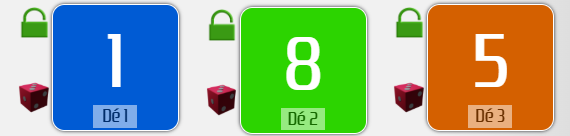
\includegraphics[width=5cm]{images/image_des.png}};
                
                % Positions des nombres formés
                %\node (n1) at (-1.6,-1.3) {\Huge \textbf{1}};
                \node (n12) at (0,-1.5) {\Huge $\mathbf{1,85}$};
                \node (n22) at (2.5,-1.5) {( nombre formé )};
                
                %\node (n23) at (1.2,-1.3) {\Huge \textbf{2 3}};
                
                % Flèches reliant les dés aux chiffres correspondants
                \draw[->, thick] (-1.5,-0.55) -- (n12.north west);
                \draw[->, thick] (0.15,-0.55) -- (0.15,-1);
                \draw[->, thick] (1.8,-0.55) -- (n12.north east);
            \end{tikzpicture}
        \end{center}
        \boite{Les événements possibles :}{ 
            % Définition de la commande pour afficher un rectangle coloré à hauteur de texte
            \newcommand{\rectangle}[1]{%
                \tikz[baseline=-0.5ex] \node[draw, fill=#1, minimum width=1em, minimum height=1em, inner sep=0pt] {};%
            }
            \vspace{-0.2cm}\begin{itemize}[label=\textbf{Type}]
                \item \textbf{R}\  \rectangle{green!85!black} : \acc{Jouer immédiatement un nouveau tour}.
                \item \textbf{C}\   \rectangle{green!85!white} : \acc{Avancer d'une unité}.
                \item \textbf{M}\   \rectangle{red!85!black} : \acc{Reculer d'une unité}.
                \item \textbf{D}\   \rectangle{blue!50} : \acc{Résoudre un défi en 30 secondes}.
                \item \textbf{E}\ Toute erreur de calcul est pénalisée par un événement : \acc{Reculer d'une unité}.
            \end{itemize}
        }
    \end{multicols}%
    \vspace{-0.35cm}\boite{Fin de partie si :}{
        \begin{multicols}{2}
            \begin{itemize}[itemsep=0em,label=$\bullet$]
                \item Une équipe arrive au bout de la frise.
                \item Le temps est écoulé. 
            \end{itemize}

                \columnbreak

            \begin{itemize}[itemsep=0em,label=$\bullet$]
                \item Une équipe complète sa fiche.
            \end{itemize}
            \vspace{-0.25cm}L'équipe qui arrive le plus loin \acc{gagne}.
        \end{multicols}
    }
\end{Activite}%

\newpage


\subsection{Informations sur la frise}% Définition des constantes

\boite{Matériel :}{
    \vspace{-0.2cm}\begin{multicols}{2}
        \begin{itemize}[label=\bcoutil]
        \item Trois dés à $10$ faces ou un \href{https://www.ma-calculatrice.fr/des-virtuels-simulateur?nbre_des=3&de_couleurs_1=005BD4&de_min_1=0&de_max_1=9&de_couleurs_2=2CD400&de_min_2=0&de_max_2=9&de_couleurs_3=D46000&de_min_3=0&de_max_3=9&de_couleurs_4=000000&de_min_4=1&de_max_4=6&de_couleurs_5=000000&de_min_5=1&de_max_5=6&de_couleurs_6=000000&de_min_6=1&de_max_6=6&de_couleurs_7=000000&de_min_7=1&de_max_7=6&de_couleurs_8=000000&de_min_8=1&de_max_8=6&de_couleurs_9=000000&de_min_9=1&de_max_9=6&de_couleurs_10=000000&de_min_10=1&de_max_10=6&de_couleurs_11=000000&de_min_11=1&de_max_11=6&de_couleurs_12=000000&de_min_12=1&de_max_12=6}{simulateur}.
        \item Des \acc{curseurs} représentant chaque équipe.
        \item Des cartes \acc{défis}.
        \item Des cartes \acc{rôle}.
        
        \columnbreak

        \item Une calculatrice pour l'équipe d'arbitrage.
        \item Une \acc{frise graduée}.
        \item Une \acc{fiche équipe}.
        \item Un chronomètre : \phantom{a}\hfill \overlaychrono{15} \hfill \phantom{a}
        \end{itemize}
    \end{multicols}
}
\def\bandwidth{4.5} % Largeur d'une bande en cm
\def\bandheight{25} % Hauteur d'une bande en cm
\def\languette{0.8}
\def\echellegraphique{10}
\def\nombremax{50}
\edef\nombrepage{\fpeval{round(\nombremax/(3*2.5),0)}}
\def\reste{1}
\begin{multicols}{2}
\begin{itemize}[label=$\bullet$]
    \item La frise suivante est à découper. 
    \item Il suffit ensuite de coller les languettes, pour assembler la frise.
    \item La frise est composée de $\num{\fpeval{(\nombrepage-\reste)*3+2}}$ morceaux répartis sur $\num{\nombrepage}$ pages.
    \item Longueur totale : $\num{\fpeval{(\bandheight * (\nombrepage - \reste) * 3 +\bandheight * 2 )  / 100}}$ m.
\end{itemize}

\columnbreak

La répartition des \acc{événements} est générée comme suit : 
\begin{center}
    \begin{tcbtab}{c|c|c|c|c}
        Type & R & C & M & D \\
        \hline
        Probabilité & $\frac{1}{6}$ & $\frac{1}{6}$ & $\frac{1}{6}$ & $\frac{1}{2}$\\
    \end{tcbtab}
\end{center}
\end{multicols}

\begin{Exemple}[Fonctionnement d'un tour de jeu]
    \vspace{-0.3cm}\begin{multicols}{2}
        \begin{enumerate}[itemsep=0em]
            \item L'équipe commence son tour à l'\acc{abscisse} $\num{7.45}$.
            \item Les élèves obtiennent, \acc{dans l'ordre} $4$, $1$ et $6$. 
            \item Le responsable complète la \acc{fiche d'avancement} avec le nombre $\num{4.16}$.
            \item L'équipe complète le résultat par $\num{7.45} + \num{4.16} = \num{\fpeval{7.45+4.16}}$.
            \item Le résultat est validé par l'équipe arbitre qui a le droit d'utiliser la calculatrice. 
            \item L'équipe tombe sur une case notée \frquote{Défi}. \\
            L'équipe pioche une carte \frquote{défi} de difficulté $2$ et répond à la question correctement.
            \item Les arbitres valident la solution. L'équipe avance de $2$ unités supplémentaires et note cette étape dans la \acc{fiche d'avancement}.
        \end{enumerate}

    \end{multicols}

    \begin{tcbtab}[Extrait de la fiche d'avancement]{c|c|c|c|c|c}
        %$\phantom{\dfrac{\dfrac{1}{10}}{\dfrac{1}{10}}}$ Tour $\phantom{\dfrac{\dfrac{1}{10}}{\dfrac{1}{10}}}$ & $1$ & $\dfrac{1}{10}$ & $\dfrac{1}{100}$ & Nombre formé & Résultat \\
        Action \no & Dé \no 1 & Dé \no 2 & Dé \no 3 & Nombre formé & Résultat \\
        \hline
        \repsim[1cm]{}  & \repsim{X} & \repsim{X} & \repsim{X} & \repsim[3cm]{X} & \repsim[6cm]{$\num{7.45}$}\\
        \hline
        \repsim[1cm]{}  & \repsim{$4$} & \repsim{$1$} & \repsim{$6$} & \repsim[3cm]{$\num{4.16}$} & \repsim[6cm]{$\num{7.45} + \num{4.16} = \num{\fpeval{7.45+4.16}}$}\\
        \hline
        \repsim[1cm]{}  & \repsim{X} & \repsim{X} & \repsim{X} & \repsim[3cm]{2} & \repsim[6cm]{$\num{\fpeval{7.45+4.16}} + 2 = \num{\fpeval{7.45+4.16+2}}$}\\
        \hline
        
    \end{tcbtab}

\end{Exemple}

\newpage



\section{Le matériel de la course aux nombres}

\subsection{Cartes de rôles}
\newcommand{\rolecard}[2]{%
  \begin{tcolorbox}[
    enhanced,
    width=7cm,
    colback=blue!10!white,
    colframe=blue!50!black,
    boxrule=1mm,
    arc=5mm,
    drop shadow={xshift=2mm,yshift=-2mm,opacity=0.5},
    fontupper=\small,
    fonttitle=\bfseries\Large,
    coltitle=white,
    colbacktitle=blue!50!black,
    title={#1},
    attach boxed title to top center={yshift=-3mm},
    boxed title style={
      sharp corners,
      boxrule=0mm,
      interior style={left color=blue!50!black, right color=blue!30!white}
    },
    overlay={%
      % Petit cercle en haut à gauche
      \draw[fill=yellow!80!orange, draw=yellow!50!red, line width=0.5mm] 
        ([xshift=-2mm,yshift=-2mm]frame.north west) circle (3mm);
      % Petit cercle en haut à droite
      \draw[fill=yellow!80!orange, draw=yellow!50!red, line width=0.5mm] 
        ([xshift=2mm,yshift=-2mm]frame.north east) circle (3mm);
      % Une étoile décorative centrée en haut
      \node[rotate=15, scale=1.2] at ([yshift=-1cm]frame.north) {\faStar};
    }
  ]
    #2
  \end{tcolorbox}
}



\begin{multicols}{2}
    \rolecard{Joueur 1}{
        \begin{center}\acc{Responsable des dés}\end{center}
        \begin{itemize}[label=\faPen]
            \item Lance trois dés à 10 faces au début de chaque tour.
            \item S'il les lance plusieurs fois d'affilée, le tour de l'équipe est annulé.
            \item Participe aux calculs en collaboration avec l'équipe.
            \item Participe à la résolution de problèmes.
        \end{itemize}
    }

    \rolecard{Joueur 2}{
        \begin{center}\acc{Responsable de la fiche}\end{center}
        \begin{itemize}[label=\faPen]
            \item Note le nombre formé en utilisant les valeurs obtenues avec les dés.
            \item Ajoute ce nombre au résultat précédent.
            \item Participe aux calculs en collaboration avec l'équipe.
            \item Participe à la résolution de problèmes.        
        \end{itemize}
    }
\end{multicols}

\vspace{3cm}

\begin{multicols}{2}

    \rolecard{Joueur 3}{
        \begin{center}\acc{Responsable du curseur}\end{center}
        \begin{itemize}[label=\faPen]
            \item Déplace le curseur sur la frise graduée en fonction du résultat.
            \item Vérifie si l'équipe atterrit sur un événement particulier.
            \item Participe aux calculs en collaboration avec l'équipe.
            \item Participe à la résolution de problèmes.
        \end{itemize}
    }

    \rolecard{Joueur 4}{
        \begin{center}\acc{Responsable de la communication}\end{center}
        \begin{itemize}[label=\faPen]
            \item Informe l'équipe des règles et des événements déclenchés.
            \item Vérifie et annonce les actions à réaliser en fonction des cases atteintes.
            \item Participe aux calculs en collaboration avec l'équipe.
            \item Participe à la résolution de problèmes.
        \end{itemize}
    }
\end{multicols}

\newpage

\begin{multicols}{2}
    \rolecard{Arbitre}{
        \begin{center}\phantom{a}\end{center}
        \begin{itemize}[label=\faPen]
            \item Valide les calculs des équipes en utilisant la calculatrice.
            \item Chronomètre les défis ( 30 secondes à 1 minute ).
            \item Peut \acc{mettre en pause} la partie à tout moment.
            \item Peut \acc{annuler une action} s'il estime que l'équipe n'est pas correcte. \\ ( triche, antijeu, moqueries...)
            \item Demande l'intervention du professeur en cas de problème.
        \end{itemize}
    }

    \columnbreak

    \rolecard{Arbitre}{
        \begin{center}\phantom{a}\end{center}
        \begin{itemize}[label=\faPen]
            \item Valide les calculs des équipes en utilisant la calculatrice.
            \item Chronomètre les défis ( 30 secondes à 1 minute ).
            \item Peut \acc{mettre en pause} la partie à tout moment.
            \item Peut \acc{annuler une action} s'il estime que l'équipe n'est pas correcte. \\ ( triche, antijeu, moqueries...)
            \item Demande l'intervention du professeur en cas de problème.
        \end{itemize}
    }
\end{multicols}

% Commande pour dessiner une case à cocher vide.
\newcommand{\hereismycheckbox}{%
  \tikz[scale=0.8] \draw[thick] (0,0) rectangle (0.4,0.4);%
}

\begin{center}
    % Le tableau comporte une première colonne pour le libellé puis 6 colonnes (3 pour chaque équipe)
    \begin{tcbtab}{p{5cm} |*{3}{>{\centering\arraybackslash}p{1.5cm}} |*{3}{>{\centering\arraybackslash}p{1.5cm}}}
      \hline
      \multirow{2}{*}{\centering\textbf{Infractions}} & \multicolumn{3}{c|}{\textbf{Équipe \no\repsim[1cm]{}}} & \multicolumn{3}{c|}{\textbf{Équipe \no\repsim[1cm]{}}} \\
      \cline{2-7}
      & \textbf{Niv. 1} & \textbf{Niv. 2} & \textbf{Niv. 3} & \textbf{Niv. 1} & \textbf{Niv. 2} & \textbf{Niv. 3} \\
      \hline
      % Exemple de ligne d'infraction avec 3 cases par équipe
      Triche aux dés & \hereismycheckbox & \hereismycheckbox & \hereismycheckbox & \hereismycheckbox & \hereismycheckbox & \hereismycheckbox \\
      \hline
      % Ajoutez ici d'autres infractions
      Retarder l'activité & \hereismycheckbox & \hereismycheckbox & \hereismycheckbox & \hereismycheckbox & \hereismycheckbox & \hereismycheckbox \\
      \hline
      Bavardages excessifs & \hereismycheckbox & \hereismycheckbox & \hereismycheckbox & \hereismycheckbox & \hereismycheckbox & \hereismycheckbox \\
      \hline
      Non-respect des consignes & \hereismycheckbox & \hereismycheckbox & \hereismycheckbox & \hereismycheckbox & \hereismycheckbox & \hereismycheckbox \\
      \hline
      Dégrade le matériel & \hereismycheckbox & \hereismycheckbox & \hereismycheckbox & \hereismycheckbox & \hereismycheckbox & \hereismycheckbox \\
      \hline
      Ne respecte pas l'arbitre & \hereismycheckbox & \hereismycheckbox & \hereismycheckbox & \hereismycheckbox & \hereismycheckbox & \hereismycheckbox \\
      \hline
    \end{tcbtab}
  \end{center}

  Observations : 

  \begin{crep}[extra lines=5]
    \phantom{a}

  \end{crep}

   \vspace{3cm}

\subsection{Fiche d'avancement}

\newpage

\chapitre[
    $\mathbf{6^{\text{ème}}}$% : $\mathbf{6^{\text{ème}}}$,$\mathbf{5^{\text{ème}}}$,$\mathbf{4^{\text{ème}}}$,$\mathbf{3^{\text{ème}}}$,$\mathbf{2^{\text{nde}}}$,$\mathbf{1^{\text{ère}}}$,$\mathbf{T^{\text{Le}}}$,
    ]{
    % : ,Equations
    }{
    Collège% : Collège,Lycée
    }{
    Amadis Jamyn% : Amadis Jamyn,Eugène Belgrand
    }{
    % : ,\tableauPresenteEvalSixieme{}{10},\tableofcontents
    }{
        Fiche d'avancement% : Exercices
    }
\setcounter{tourcounter}{0}
\vspace{-0.8cm}\begin{center}
    \begin{tcbtab}{c|c|c|c|c}
        \'Equipe \no\repsim[1cm]{}& Joueur 1 & Joueur 2 & Joueur 3 & Joueur 4\\
        \hline
        Nom & \repsim[3.3cm]{} & \repsim[3.3cm]{} & \repsim[3.3cm]{} & \repsim[3.3cm]{}\\
        \hline
        Responsable de : & Dés & Fiche d'avancement & Curseur & Communication \\
    \end{tcbtab}
\end{center}
\vspace{-0.8cm}\begin{center}
    \begin{tcbtab}{c|c|c|c|c|c}
        %$\phantom{\dfrac{\dfrac{1}{10}}{\dfrac{1}{10}}}$ Tour $\phantom{\dfrac{\dfrac{1}{10}}{\dfrac{1}{10}}}$ & $1$ & $\dfrac{1}{10}$ & $\dfrac{1}{100}$ & Nombre formé & Résultat \\
        Action \no & Dé \no 1 & Dé \no 2 & Dé \no 3 & Nombre formé & Résultat \\
        \hline
        \repsim[1cm]{}  & \repsim{} & \repsim{} & \repsim{} & \repsim[3cm]{} & \repsim[6cm]{}\\
        \hline
        \repsim[1cm]{}  & \repsim{} & \repsim{} & \repsim{} & \repsim[3cm]{} & \repsim[6cm]{}\\
        \hline
        \repsim[1cm]{}  & \repsim{} & \repsim{} & \repsim{} & \repsim[3cm]{} & \repsim[6cm]{}\\
        \hline
        \repsim[1cm]{}  & \repsim{} & \repsim{} & \repsim{} & \repsim[3cm]{} & \repsim[6cm]{}\\
        \hline
        \repsim[1cm]{}  & \repsim{} & \repsim{} & \repsim{} & \repsim[3cm]{} & \repsim[6cm]{}\\
        \hline
        \repsim[1cm]{}  & \repsim{} & \repsim{} & \repsim{} & \repsim[3cm]{} & \repsim[6cm]{}\\
        \hline
        \repsim[1cm]{}  & \repsim{} & \repsim{} & \repsim{} & \repsim[3cm]{} & \repsim[6cm]{}\\
        \hline
        \repsim[1cm]{}  & \repsim{} & \repsim{} & \repsim{} & \repsim[3cm]{} & \repsim[6cm]{}\\
        \hline
        \repsim[1cm]{}  & \repsim{} & \repsim{} & \repsim{} & \repsim[3cm]{} & \repsim[6cm]{}\\
        \hline
        \repsim[1cm]{}  & \repsim{} & \repsim{} & \repsim{} & \repsim[3cm]{} & \repsim[6cm]{}\\
        \hline
        \repsim[1cm]{}  & \repsim{} & \repsim{} & \repsim{} & \repsim[3cm]{} & \repsim[6cm]{}\\
        \hline
        \repsim[1cm]{}  & \repsim{} & \repsim{} & \repsim{} & \repsim[3cm]{} & \repsim[6cm]{}\\
        \hline
        \repsim[1cm]{}  & \repsim{} & \repsim{} & \repsim{} & \repsim[3cm]{} & \repsim[6cm]{}\\
        \hline
        \repsim[1cm]{}  & \repsim{} & \repsim{} & \repsim{} & \repsim[3cm]{} & \repsim[6cm]{}\\
        \hline
        \repsim[1cm]{}  & \repsim{} & \repsim{} & \repsim{} & \repsim[3cm]{} & \repsim[6cm]{}\\
        \hline
        \repsim[1cm]{}  & \repsim{} & \repsim{} & \repsim{} & \repsim[3cm]{} & \repsim[6cm]{}\\
        \hline
        \repsim[1cm]{}  & \repsim{} & \repsim{} & \repsim{} & \repsim[3cm]{} & \repsim[6cm]{}\\
        \hline
        \repsim[1cm]{}  & \repsim{} & \repsim{} & \repsim{} & \repsim[3cm]{} & \repsim[6cm]{}\\
        \hline
        \repsim[1cm]{}  & \repsim{} & \repsim{} & \repsim{} & \repsim[3cm]{} & \repsim[6cm]{}\\
        \hline
        \repsim[1cm]{}  & \repsim{} & \repsim{} & \repsim{} & \repsim[3cm]{} & \repsim[6cm]{}
    \end{tcbtab}        
\end{center}

\newcommand{\drawGraduations}[3]{%
    % #1: Start value
    % #2: End value
    % #3: Offset value (for continuity)

    % Centièmes graduations (réduction du nombre de graduations)
    \def\scalefactor{1}

    \foreach \x in {#1,0.1,...,#2} {
        \draw[very thick] (0,\x*\scalefactor) -- (0.6, \x*\scalefactor);
    }

    % Dixièmes graduations
    \foreach \x in {#1,1,...,#2} {
        \draw[very thick] (0,\x*\scalefactor) -- (1.5, \x*\scalefactor);
    }

    % Unités graduations et affichage en grand et gras pour les entiers
    \foreach \x in {#1,1,...,\fpeval{#2+0.1}} {
        \draw[very thick] (0,\x*\scalefactor) -- (1.5, \x*\scalefactor);
        \pgfmathsetmacro{\value}{(\x + #3) / 10}
        \pgfmathsetmacro{\semivalue}{(\x + #3 + 5) / 10}
        \pgfmathsetmacro{\semiremainder}{mod(\semivalue,1)}
        \pgfmathsetmacro{\remainder}{mod(\value,1)}
        \ifdim \remainder pt = 0pt
            \node[left, font=\bfseries\LARGE] at (0, \x*\scalefactor) {\fpeval{\value}};
        \fi
        \ifdim \semiremainder pt = 0pt
            \node[left, font=\bfseries\large] at (0, \x*\scalefactor) {\num{\fpeval{\value}}};
        \fi
    }

        % Gamification : ajouter des événements aléatoires
        \pgfmathsetmacro{\randomShift}{rnd*4 - 2} % Générer une variation entre -2 et +2
        \pgfmathsetmacro{\eventCount}{int(5 + \randomShift)} % Base 5 événements avec une variation de -2 à +2
        \foreach \i in {1,...,\eventCount} {
        \pgfmathsetmacro{\randY}{random(\fpeval{#1},\fpeval{#2 - 3})}
        \pgfmathrandominteger{\randheight}{1}{2}
        \pgfmathsetmacro{\randX}{0.5*\bandwidth}
        \pgfmathrandominteger{\eventType}{1}{6}
        \def\eventcolor{yellow}
        \def\eventTextColor{black}
        % Définition des labels selon l'événement
        \ifnum\eventType=1
            \def\eventText{R}%Relancer les dés
            \def\eventcolor{green!85!black}
        \fi
        \ifnum\eventType=2
            \def\eventText{D}%Défi}
            \def\eventcolor{blue!35!white}
        \fi
        \ifnum\eventType=3
            \def\eventText{C}%Événement chanceux}
            \def\eventcolor{green!75!white}
        \fi
        \ifnum\eventType=4
            \def\eventText{D}%Défi}
            \def\eventcolor{blue!35!white}
        \fi
        \ifnum\eventType=5
            \def\eventText{M}%Événement malchanceux}
            \def\eventcolor{red!85!black}
            \def\eventTextColor{white}
        \fi
        \ifnum\eventType=6
            \def\eventText{D}%Défi}
            \def\eventcolor{blue!35!white}%green!75!white}
        \fi
        % Dessiner l'événement à une position aléatoire
        \draw[fill=\eventcolor, rounded corners] (\randX, \randY) rectangle ++(2, \randheight+1);

        % Calcul de l'intervalle et placement des labels
        \pgfmathsetmacro{\startY}{\randY}
        \pgfmathsetmacro{\endY}{\randY + \randheight}
        \foreach \y in {\startY, \fpeval{\startY + 1}, ..., \endY} {
            \node at (\randX + 1, \y + 0.5) {\LARGE{\textbf{\color{\eventTextColor}\eventText}}};
        }
    }
    
    % Languette de collage pour lier à la frise suivante
    \draw[thick, fill=gray!30] (0, \bandheight) rectangle (\bandwidth, \bandheight + \languette);
    \node[above, font=\small] at (\bandwidth/2, \bandheight + \languette / 10) {Languette de collage};
}





\subsection{Les curseurs}


\vspace{1.5cm}\begin{center}
    \curseur{blue}{1} \hspace{1cm} \curseur{red}{2} \hspace{1cm} \curseur{green}{3}
\end{center}

\vspace{1.5cm}\begin{center}
    \curseur{yellow}{4} \hspace{1cm} \curseur{purple}{5}
\end{center}

\subsection{Tutoriel}

\newpage

\def\bandwidth{4.5} % Largeur d'une bande en cm
\def\bandheight{25} % Hauteur d'une bande en cm
\def\languette{0.8}
\def\echellegraphique{10}
\def\nombremax{50}
\edef\nombrepage{\fpeval{round(\nombremax/(3*2.5),0)}}
\def\reste{1}
\newcommand{\drawTutoGraduations}[3]{%
    % #1: Start value
    % #2: End value
    % #3: Offset value (for continuity)

    % Centièmes graduations (réduction du nombre de graduations)
    \def\scalefactor{1}

    \foreach \x in {#1,0.1,...,#2} {
        \draw[very thick] (0,\x*\scalefactor) -- (0.6, \x*\scalefactor);
    }

    % Dixièmes graduations
    \foreach \x in {#1,1,...,#2} {
        \draw[very thick] (0,\x*\scalefactor) -- (1.5, \x*\scalefactor);
    }

    % Unités graduations et affichage en grand et gras pour les entiers
    \foreach \x in {#1,1,...,\fpeval{#2+0.1}} {
        \draw[very thick] (0,\x*\scalefactor) -- (1.5, \x*\scalefactor);
        \pgfmathsetmacro{\value}{(\x + #3) / 10}
        \pgfmathsetmacro{\semivalue}{(\x + #3 + 5) / 10}
        \pgfmathsetmacro{\semiremainder}{mod(\semivalue,1)}
        \pgfmathsetmacro{\remainder}{mod(\value,1)}
        \ifdim \remainder pt = 0pt
            \node[left, font=\bfseries\LARGE] at (0, \x*\scalefactor) {\fpeval{\value}};
        \fi
        \ifdim \semiremainder pt = 0pt
            \node[left, font=\bfseries\large] at (0, \x*\scalefactor) {\num{\fpeval{\value}}};
        \fi
    }

        % Gamification : ajouter des événements aléatoires
        \pgfmathsetmacro{\randomShift}{rnd*4 - 2} % Générer une variation entre -2 et +2
        \pgfmathsetmacro{\eventCount}{int(5 + \randomShift)} % Base 5 événements avec une variation de -2 à +2
        \foreach \i in {1,...,\eventCount} {
        \pgfmathsetmacro{\randY}{random(\fpeval{#1},\fpeval{#2 - 3})}
        \pgfmathrandominteger{\randheight}{1}{2}
        \pgfmathsetmacro{\randX}{0.5*\bandwidth}
        \pgfmathrandominteger{\eventType}{1}{6}
        \def\eventcolor{yellow}
        \def\eventTextColor{black}
        % Définition des labels selon l'événement
        \ifnum\eventType=1
            \def\eventText{R}%Relancer les dés
            \def\eventcolor{green!85!black}
        \fi
        \ifnum\eventType=2
            \def\eventText{M}%Événement malchanceux}
            \def\eventcolor{red!85!black}
            \def\eventTextColor{white}
        \fi
        \ifnum\eventType=3
            \def\eventText{C}%Événement chanceux}
            \def\eventcolor{green!75!white}
        \fi
        \ifnum\eventType=4
            \def\eventText{D}%Défi}
            \def\eventcolor{blue!35!white}
        \fi
        \ifnum\eventType=5
            \def\eventText{D}%Défi}
            \def\eventcolor{blue!35!white}
        \fi
        \ifnum\eventType=6
            \def\eventText{D}%Défi}
            \def\eventcolor{blue!35!white}%green!75!white}
        \fi
        % Dessiner l'événement à une position aléatoire
        \draw[fill=\eventcolor, rounded corners] (\randX, \randY) rectangle ++(2, \randheight+1);

        % Calcul de l'intervalle et placement des labels
        \pgfmathsetmacro{\startY}{\randY}
        \pgfmathsetmacro{\endY}{\randY + \randheight}
        \foreach \y in {\startY, \fpeval{\startY + 1}, ..., \endY} {
            \node at (\randX + 1, \y + 0.5) {\LARGE{\textbf{\color{\eventTextColor}\eventText}}};
        }
    }
    
    % Languette de collage pour lier à la frise suivante
    \draw[thick, fill=gray!30] (0, \bandheight) rectangle (\bandwidth, \bandheight + \languette);
    \node[above, font=\small] at (\bandwidth/2, \bandheight + \languette / 10) {Languette de collage};
}

% Votre commande de grille (adaptée ou existante)
\newcommand{\drawTutoGraduationsFixed}[4]{%
    % #1: valeur de début, #2: valeur de fin, #3: décalage numérique, #4: shift (position de la grille)
    \begin{scope}[shift={#4}]
        \def\scalefactor{1}
        
        % Tracé des graduations centièmes et dixièmes (exemple simplifié)
        \foreach \x in {#1,0.1,...,#2} {
            \draw[very thick] (0,\x*\scalefactor) -- (0.6,\x*\scalefactor);
        }
        \foreach \x in {#1,1,...,#2} {
            \draw[very thick] (0,\x*\scalefactor) -- (1.5,\x*\scalefactor);
        }
        % Unités graduations et affichage en grand et gras pour les entiers
        \foreach \x in {#1,1,...,\fpeval{#2+0.1}} {
            \draw[very thick] (0,\x*\scalefactor) -- (1.5, \x*\scalefactor);
            \pgfmathsetmacro{\value}{(\x + #3) / 10}
            \pgfmathsetmacro{\semivalue}{(\x + #3 + 5) / 10}
            \pgfmathsetmacro{\semiremainder}{mod(\semivalue,1)}
            \pgfmathsetmacro{\remainder}{mod(\value,1)}
            \ifdim \remainder pt = 0pt
                \node[left, font=\bfseries\LARGE] at (0, \x*\scalefactor) {\fpeval{\value}};
            \fi
            \ifdim \semiremainder pt = 0pt
                \node[left, font=\bfseries\large] at (0, \x*\scalefactor) {\num{\fpeval{\value}}};
            \fi
        }
    \end{scope}
}

% Commande pour dessiner les événements fixes sur la frise
\newcommand{\drawFixedEvents}{%
  \def\eventx{0.5*\bandwidth}%
  % Événement 1 : Défi (9 à 11)
  \draw[fill=blue!35, rounded corners] (\eventx,10) rectangle ++(2,2);
  \node at ($(\eventx,10)!0.5!(\eventx+2,12)$) {\LARGE \textbf{D}};
  % Événement 2 : Chanceux (12 à 13)
  \draw[fill=green!75!white, rounded corners] (\eventx,12) rectangle ++(2,1);
  \node at ($(\eventx,12)!0.5!(\eventx+2,13)$) {\LARGE \textbf{C}};
  % Événement 3 : Autre défi (15 à 17)
  \draw[fill=blue!35, rounded corners] (\eventx,15) rectangle ++(2,2);
  \node at ($(\eventx,15)!0.5!(\eventx+2,17)$) {\LARGE \textbf{D}};
  % Événement 4 : Malchanceux (21 à 23)
  \draw[fill=red!85!black, rounded corners] (\eventx,21) rectangle ++(2,2);
  \node at ($(\eventx,21)!0.5!(\eventx+2,23)$) {\LARGE \textbf{\color{white}M}};
  % Événement 5 : Relance (28 à 31)
  \draw[fill=green!85!black, rounded corners] (\eventx,28) rectangle ++(2,3);
  \node at ($(\eventx,28)!0.5!(\eventx+2,31)$) {\LARGE \textbf{R}};
}


\newcommand{\placecurseurAt}[4]{%
    % #1 : Couleur du curseur
    % #2 : Numéro de l'équipe
    % #3 : Coordonnée x
    % #4 : Coordonnée y
    \begin{scope}[shift={(#3,#4)}]
         % Flèche tournée vers la droite (miroir de celle d'origine)
         \fill[#1] (2,0) -- (0,1) -- (0.5,0) -- (0,-1) -- cycle;
         \draw[thick, black] (2,0) -- (0,1) -- (0.5,0) -- (0,-1) -- cycle;
         
         % Bulle (positionnée à gauche de la flèche)
         \fill[#1!50] (-0.5,0) circle (1);
         \draw[thick, black] (-0.5,0) circle (1);
         
         % Queue reliant la bulle (placée sur le côté droit de la bulle)
         \fill[#1!50] (0,0) -- (-0.2,-0.2) -- (-0.4,0.1) -- cycle;
         
         % Texte dans la bulle
         \node at (-0.5,0) {\textbf{\Huge #2}};

         % Position pour le tuto
         \draw[line width=2pt, #1!65!black, dashed] (2,0) -- (2+\bandwidth,0);

         % abscisse du curseur
         \node at (3+\bandwidth,0) {\color{#1!85!black} \Huge $\mathbf{\num{\fpeval{#4 / 10}}}$};
    \end{scope}
}
\newcommand{\flechedeplacement}[3]{%
  \begin{scope}
    % Paramètres de la flèche
    \def\arrowThickness{0.6} % épaisseur de la flèche en cm
    \def\arrowHead{0.5}      % hauteur de la pointe en cm
    
    % Calcul de la moitié de l'épaisseur pour centrer la flèche sur l'axe horizontal
    \pgfmathsetmacro{\halfThickness}{\arrowThickness/2}%
    % Position horizontale centrée sur la frise (en supposant que \bandwidth est défini)
    \pgfmathsetmacro{\xcenter}{\bandwidth/2}%
    % Position pour le tuto
    \draw[line width=2pt, #1!65!black, dashed] (0,#2) -- (\bandwidth,#2);

    % abscisse du curseur
    \node at (1 +\bandwidth,#2) {\color{#1!85!black} \Huge $\mathbf{\num{\fpeval{#2 / 10}}}$};
    % distance parcourue
    \pgfmathsetmacro{\ycoord}{(#2+#3)/2}%
    \node at (2+\bandwidth,\ycoord) {\color{#1!85!black} \Huge $\mathbf{+\num{\fpeval{(#3 - #2)/10}}}$};
    
    % Dessin de la flèche (forme de polygone)
    \filldraw[fill={#1!50!white}, draw=black, line width=1pt]
         (\xcenter - \halfThickness, #2) --
         (\xcenter + \halfThickness, #2) --
         (\xcenter + \halfThickness, {#3 - \arrowHead}) --
         (\xcenter, #3) --
         (\xcenter - \halfThickness, {#3 - \arrowHead}) -- cycle;
  \end{scope}%
}
\newcommand{\flecherecul}[3]{%
  \begin{scope}
    % Paramètres de la flèche
    \def\arrowThickness{0.6} % épaisseur de la flèche en cm
    \def\arrowHead{0.5}      % hauteur de la pointe en cm
    
    % Calcul de la moitié de l'épaisseur (pour centrer la flèche horizontalement)
    \pgfmathsetmacro{\halfThickness}{\arrowThickness/2}%
    % Position horizontale centrée sur la frise (on suppose que \bandwidth est défini)
    \pgfmathsetmacro{\xcenter}{\bandwidth/2}%
    % Position pour la ligne horizontale ( départ )
    \draw[line width=2pt, #1!65!black, dashed] (0,#2) -- (\bandwidth,#2);
    % abscisse du départ
    \node at (1+\bandwidth,#2) {\color{#1!85!black} \Huge $\mathbf{\num{\fpeval{#2 / 10}}}$};
    % distance parcourue
    \pgfmathsetmacro{\ycoord}{(#2+#3)/2}%
    \node at (2+\bandwidth,\ycoord) {\color{#1!85!black} \Huge $\mathbf{-\num{\fpeval{(#2 - #3)/10}}}$};
        % Construction de la flèche inversée (point en bas)
    \filldraw[fill={#1!50!white}, draw=black, line width=1pt]
         % Partie supérieure du rectangle
         (\xcenter - \halfThickness - 0.5, #2) --  % coin supérieur gauche
         (\xcenter + \halfThickness - 0.5, #2) --  % coin supérieur droit
         % Descente du rectangle jusqu'au début de la pointe
         (\xcenter + \halfThickness - 0.5, {#3 + \arrowHead}) -- 
         % Pointe : le sommet de la flèche (centre en bas)
         (\xcenter - 0.5, #3) -- 
         % Retour par le côté gauche
         (\xcenter - \halfThickness - 0.5, {#3 + \arrowHead}) -- 
         cycle;
  \end{scope}%
}

\begin{multicols}{2}
\begin{tikzpicture}[x=1cm, y=1cm,xshift=-0.5cm,yshift=0.5cm]

    % Dessin de la première bande
    \begin{scope}[shift={(2,1)}]
        \draw[thick] (0,0) rectangle (\bandwidth, \bandheight);
        \clip (-4,-1) rectangle (\bandwidth + 4, \bandheight+\languette+1);
        %\drawTutoGraduations{0}{25}{0}
        % Exemple d'utilisation de la commande de grille
        \drawTutoGraduationsFixed{0}{25}{0}{(0,0)}
        % Ajout des événements fixes sur la frise
        \drawFixedEvents
        \placecurseurAt{blue}{1}{-2}{10.7}
        \placecurseurAt{red}{2}{-2}{0}
        \flechedeplacement{blue}{0}{10.7}%{15}
        %\placecurseurAt{green}{3}{-2}{23}
    \end{scope}
    
    
\end{tikzpicture}

\columnbreak

\phantom{a}
\vfill
\begin{center}
    \begin{minipage}{0.7\columnwidth}
    \boite{Action \no 1 :}{
        \begin{enumerate}
            \item L'équipe \no 1 lance les dés et obtient $1$ ; $0$ et $7$.
            \item Le responsable remplit la fiche d'avancement en \acc{composant} le nombre $\num{1.07}$. 
            \item Le responsable du curseur le place sur la frise.
            \item Le responsable de la communication annonce \frquote{Pour contrôle !}
            \item L'équipe d'arbitrage valide la position.
        \end{enumerate}
    }
    \end{minipage}
\end{center}
\vfill
\phantom{a}
\end{multicols}


\newpage

\begin{multicols}{2}
    \begin{tikzpicture}[x=1cm, y=1cm,xshift=-0.5cm,yshift=0.5cm]
    
        % Dessin de la première bande
        \begin{scope}[shift={(2,1)}]
            \draw[thick] (0,0) rectangle (\bandwidth, \bandheight);
            \clip (-4,-1) rectangle (\bandwidth + 4, \bandheight+\languette+1);
            %\drawTutoGraduations{0}{25}{0}
            % Exemple d'utilisation de la commande de grille
            \drawTutoGraduationsFixed{0}{25}{0}{(0,0)}
            % Ajout des événements fixes sur la frise
            \drawFixedEvents
            \placecurseurAt{blue}{1}{-2}{20.7}
            \placecurseurAt{red}{2}{-2}{0}
            \flechedeplacement{blue}{10.7}{20.7}%\placecurseurAt{green}{3}{-2}{23}
        \end{scope}
        
        
    \end{tikzpicture}
    
    \columnbreak
    
    \phantom{a}
    \vfill
    \begin{center}
        \begin{minipage}{0.7\columnwidth}
            \boite{Action \no 2 :}{
                \begin{enumerate}
                    \item L'équipe \no 1 se trouve sur une case \frquote{Défi} : elle pioche un problème.
                    \item Elle obtient le problème de niveau 1 suivant et donne la bonne réponse.\\
                    
                    \mesTutocartes{green}{Q.1.3}{ $17+25$ }{S.1.3}{$17+25=42$}%
    
                    \item L'équipe d'arbitrage valide la réponse.
                    \item Le responsable du curseur avance d'une unité.
                    \item Le responsable de la communication annonce \frquote{Pour contrôle !}
                    \item L'équipe d'arbitrage valide la position.
                \end{enumerate}
            }
        \end{minipage}
    \end{center}
    \vfill
    \phantom{a}
    \end{multicols}
    
    
    \newpage

    \begin{multicols}{2}
        \begin{tikzpicture}[x=1cm, y=1cm,xshift=-0.5cm,yshift=0.5cm]
        
            % Dessin de la première bande
            \begin{scope}[shift={(2,1)}]
                \draw[thick] (0,0) rectangle (\bandwidth, \bandheight);
                \clip (-4,-1) rectangle (\bandwidth + 4, \bandheight+\languette+1);
                %\drawTutoGraduations{0}{25}{0}
                % Exemple d'utilisation de la commande de grille
                \drawTutoGraduationsFixed{0}{25}{0}{(0,0)}
                % Ajout des événements fixes sur la frise
                \drawFixedEvents
                \placecurseurAt{blue}{1}{-2}{20.7}
                \placecurseurAt{red}{2}{-2}{18.4}
                %\placecurseurAt{green}{3}{-2}{23}
                \flechedeplacement{red}{0}{18.4}
            \end{scope}
            
            
        \end{tikzpicture}
        
        \columnbreak
        
        \phantom{a}
        \vfill
        \begin{center}
            \begin{minipage}{0.7\columnwidth}
            \boite{Action \no 3 :}{
                \begin{enumerate}
                    \item L'équipe \no 2 lance les dés et obtient $1$ ; $8$ et $4$.
                    \item Le responsable complète la fiche d'avancement.    
                    \item Le responsable du curseur le place sur la frise.
                    \item Le responsable de la communication annonce \frquote{Pour contrôle !}
                    \item L'équipe d'arbitrage valide la position.
                \end{enumerate}
            }
            \end{minipage}
        \end{center}
        \vfill
        \phantom{a}
        \end{multicols}

\newpage

\begin{multicols}{2}
    \begin{tikzpicture}[x=1cm, y=1cm,xshift=-0.5cm,yshift=0.5cm]
    
        % Dessin de la première bande
        \begin{scope}[shift={(2,1)}]
            \draw[thick] (0,0) rectangle (\bandwidth, \bandheight);
            \clip (-4,-1) rectangle (\bandwidth + 4, \bandheight+\languette+1);
            %\drawTutoGraduations{0}{25}{0}
            % Exemple d'utilisation de la commande de grille
            \drawTutoGraduationsFixed{0}{25}{0}{(0,0)}
            % Ajout des événements fixes sur la frise
            \drawFixedEvents
            \placecurseurAt{blue}{1}{-2}{22.8}
            \placecurseurAt{red}{2}{-2}{18.4}
            %\placecurseurAt{green}{3}{-2}{23}
            \flechedeplacement{blue}{20.7}{22.8}
        \end{scope}
        
        
    \end{tikzpicture}
    
    \columnbreak
    
    \phantom{a}
    \vfill
    \begin{center}
        \begin{minipage}{0.7\columnwidth}
        \boite{Action \no 4 :}{
            \begin{enumerate}
                \item L'équipe \no 1 lance les dés et obtient $0$ ; $2$ et $1$.
                \item Le responsable complète la fiche d'avancement :
                
                $\num{2.07} + \num{0.21} = \num{\fpeval{2.07+0.21}}$
                \item Le responsable du curseur le place sur la frise.
                \item Le responsable de la communication annonce \frquote{Pour contrôle !}
                \item L'équipe d'arbitrage valide la position.
            \end{enumerate}
        }
        \end{minipage}
    \end{center}
    \vfill
    \phantom{a}
    \end{multicols}

\newpage

\begin{multicols}{2}
    \begin{tikzpicture}[x=1cm, y=1cm,xshift=-0.5cm,yshift=0.5cm]
    
        % Dessin de la première bande
        \begin{scope}[shift={(2,1)}]
            \draw[thick] (0,0) rectangle (\bandwidth, \bandheight);
            \clip (-4,-1) rectangle (\bandwidth + 4, \bandheight+\languette+1);
            %\drawTutoGraduations{0}{25}{0}
            % Exemple d'utilisation de la commande de grille
            \drawTutoGraduationsFixed{0}{25}{0}{(0,0)}
            % Ajout des événements fixes sur la frise
            \drawFixedEvents
            \placecurseurAt{blue}{1}{-2}{12.8}
            \placecurseurAt{red}{2}{-2}{18.4}
            %\placecurseurAt{green}{3}{-2}{23}
            \flecherecul{blue}{22.8}{12.8}
        \end{scope}
        
        
    \end{tikzpicture}
    
    \columnbreak
    
    \phantom{a}
    \vfill
    \begin{center}
        \begin{minipage}{0.7\columnwidth}
        \boite{Action \no 5 :}{
            \begin{enumerate}
                \item L'équipe \no 1 \acc{recule} d'une unité puisque le curseur atterit sur une case \frquote{Malchance}.
                \item Le responsable complète la fiche d'avancement.    
                \item Le responsable du curseur le place sur la frise.
                \item Le responsable de la communication annonce \frquote{Pour contrôle !}
                \item L'équipe d'arbitrage valide la position.
                \item Même si l'équipe arrive sur un événement \frquote{Chanceux}, elle ne le déclenche pas car elle a déjà eu un événement ce tour. 
            \end{enumerate}
        }
        \end{minipage}
    \end{center}
    \vfill
    \phantom{a}
    \end{multicols}

\newpage



\newpage

\subsection{La frise}

\newpage

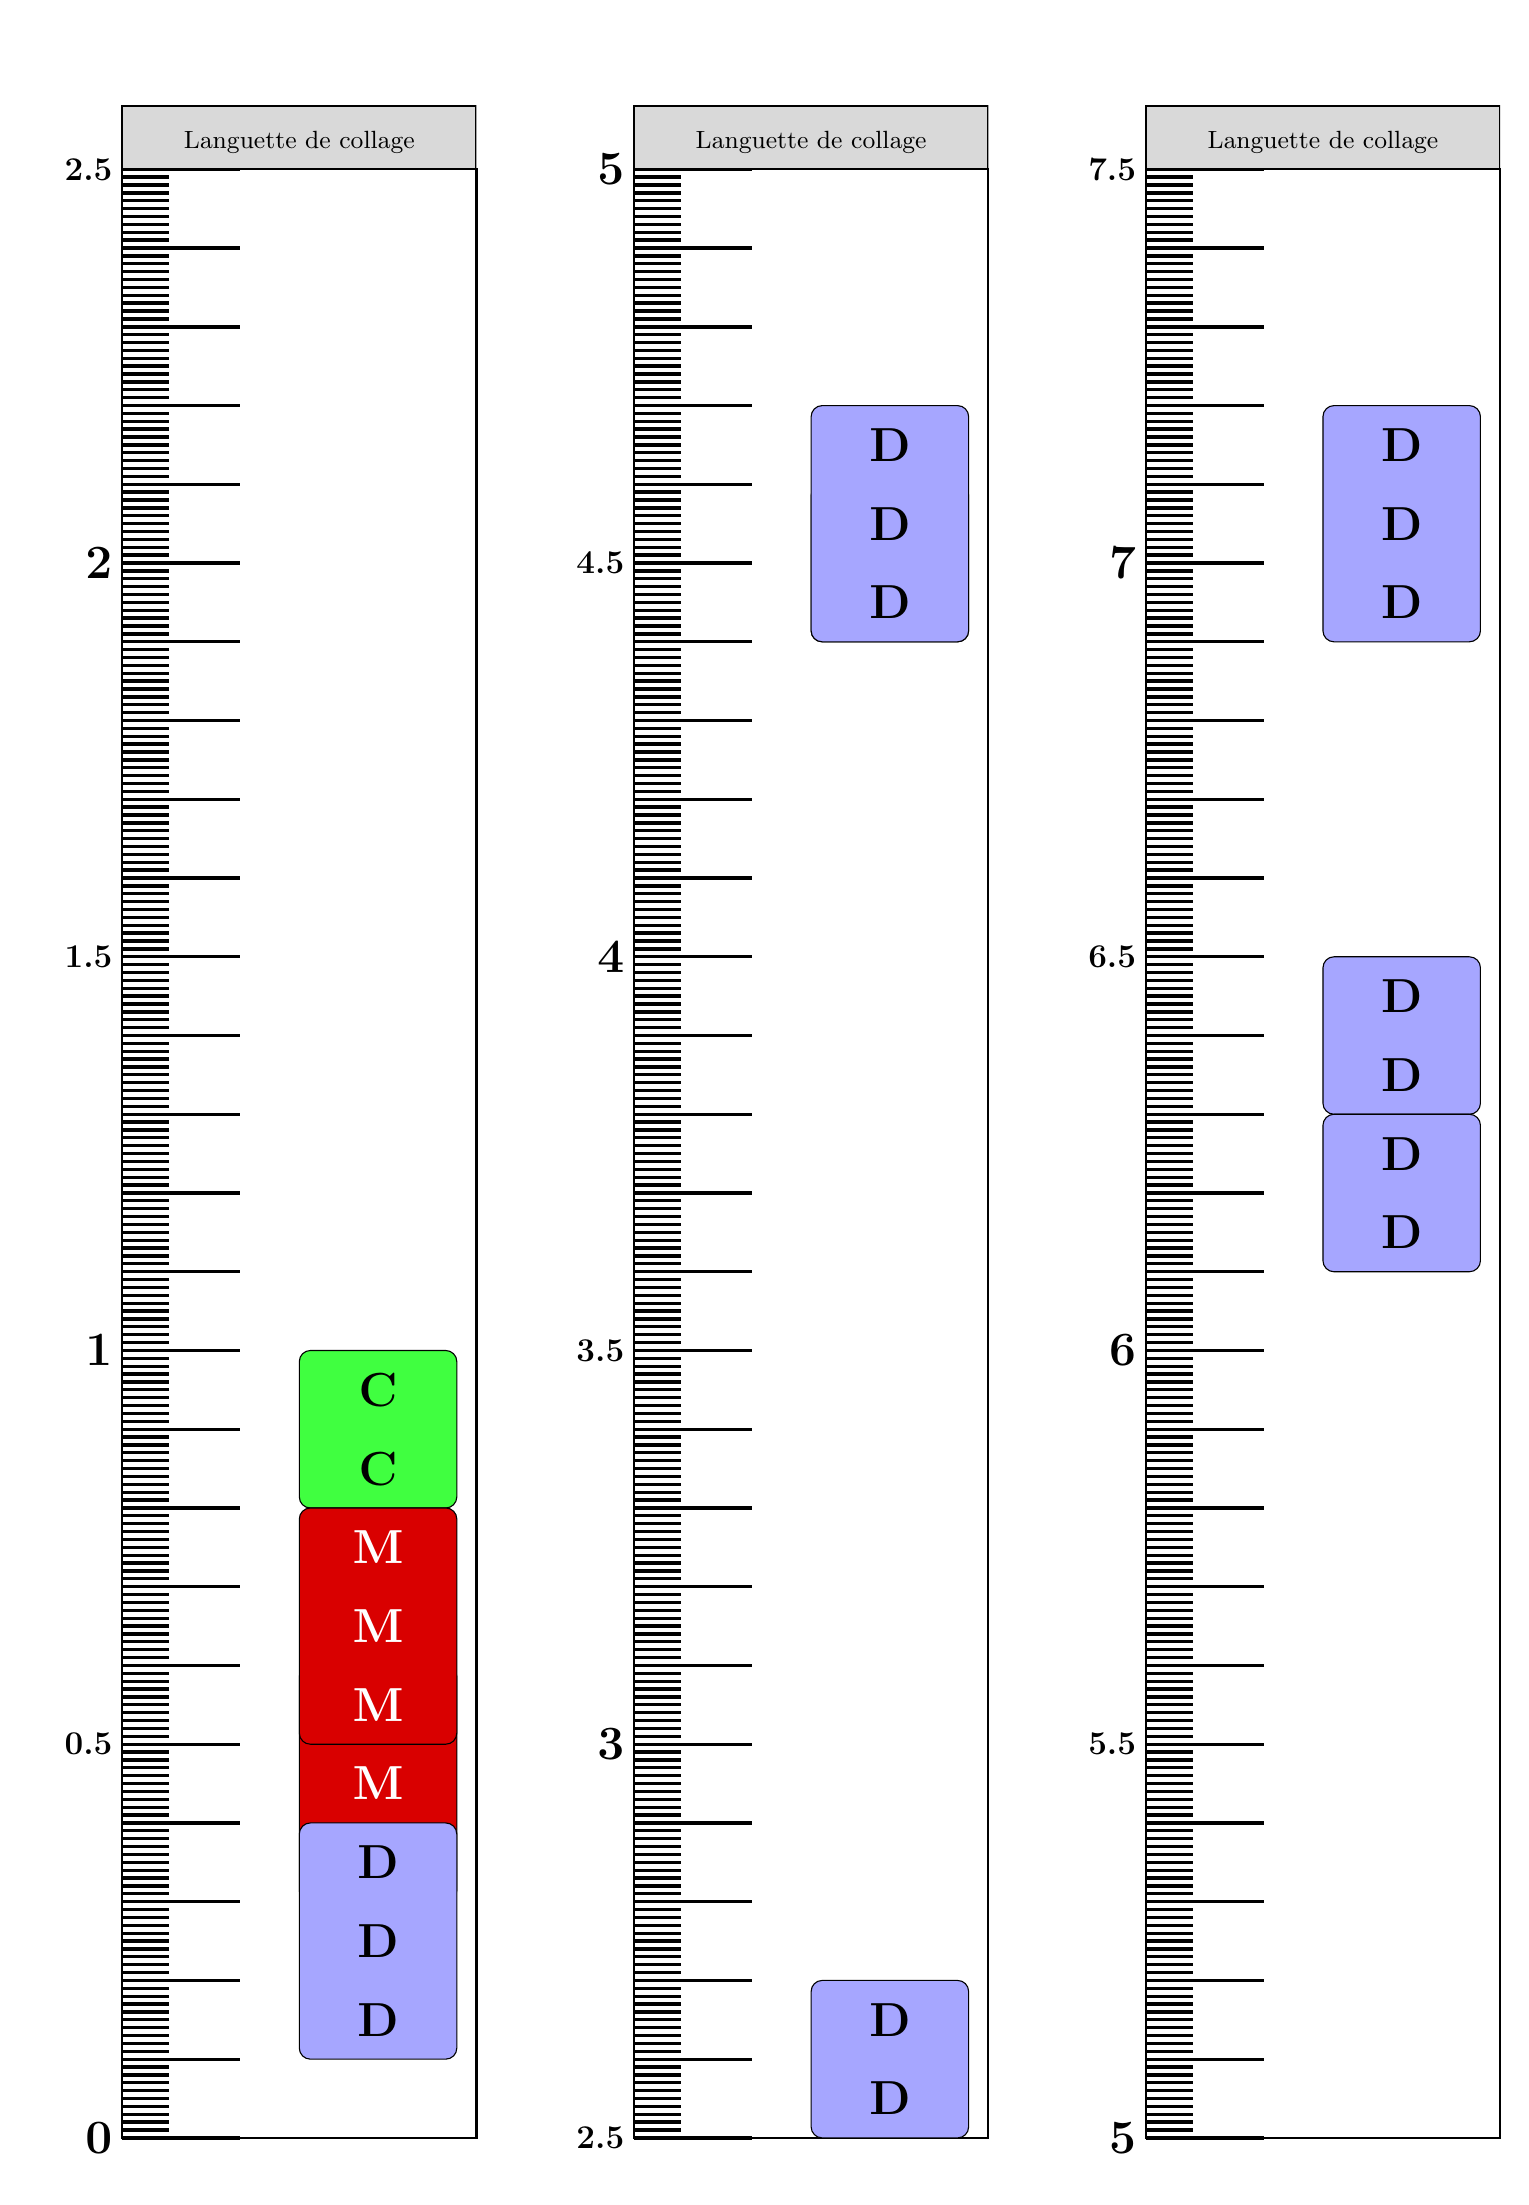
\begin{tikzpicture}[x=1cm, y=1cm,xshift=-1cm]

% Dessin de la première bande
\begin{scope}[shift={(-1,0)}]
    \draw[thick] (0,0) rectangle (\bandwidth, \bandheight);
    \clip (-1.2,-0.5) rectangle (\bandwidth, \bandheight+\languette+1);
    \drawGraduations{0}{25}{0}
\end{scope}

% Dessin de la deuxième bande (avec continuité des nombres)
\begin{scope}[shift={(1*\bandwidth + 1,0)}]
    \draw[thick] (0,0) rectangle (\bandwidth, \bandheight);
    \clip (-1.2,-0.5) rectangle (\bandwidth, \bandheight+\languette+1);
    \drawGraduations{0}{25}{25}
\end{scope}

% Dessin de la troisième bande (avec continuité des nombres)
\begin{scope}[shift={(2*\bandwidth + 3,0)}]
    \draw[thick] (0,0) rectangle (\bandwidth, \bandheight);
    \clip (-1.2,-0.5) rectangle (\bandwidth, \bandheight+\languette+1);
    \drawGraduations{0}{25}{50}
\end{scope}

\end{tikzpicture}

\newpage

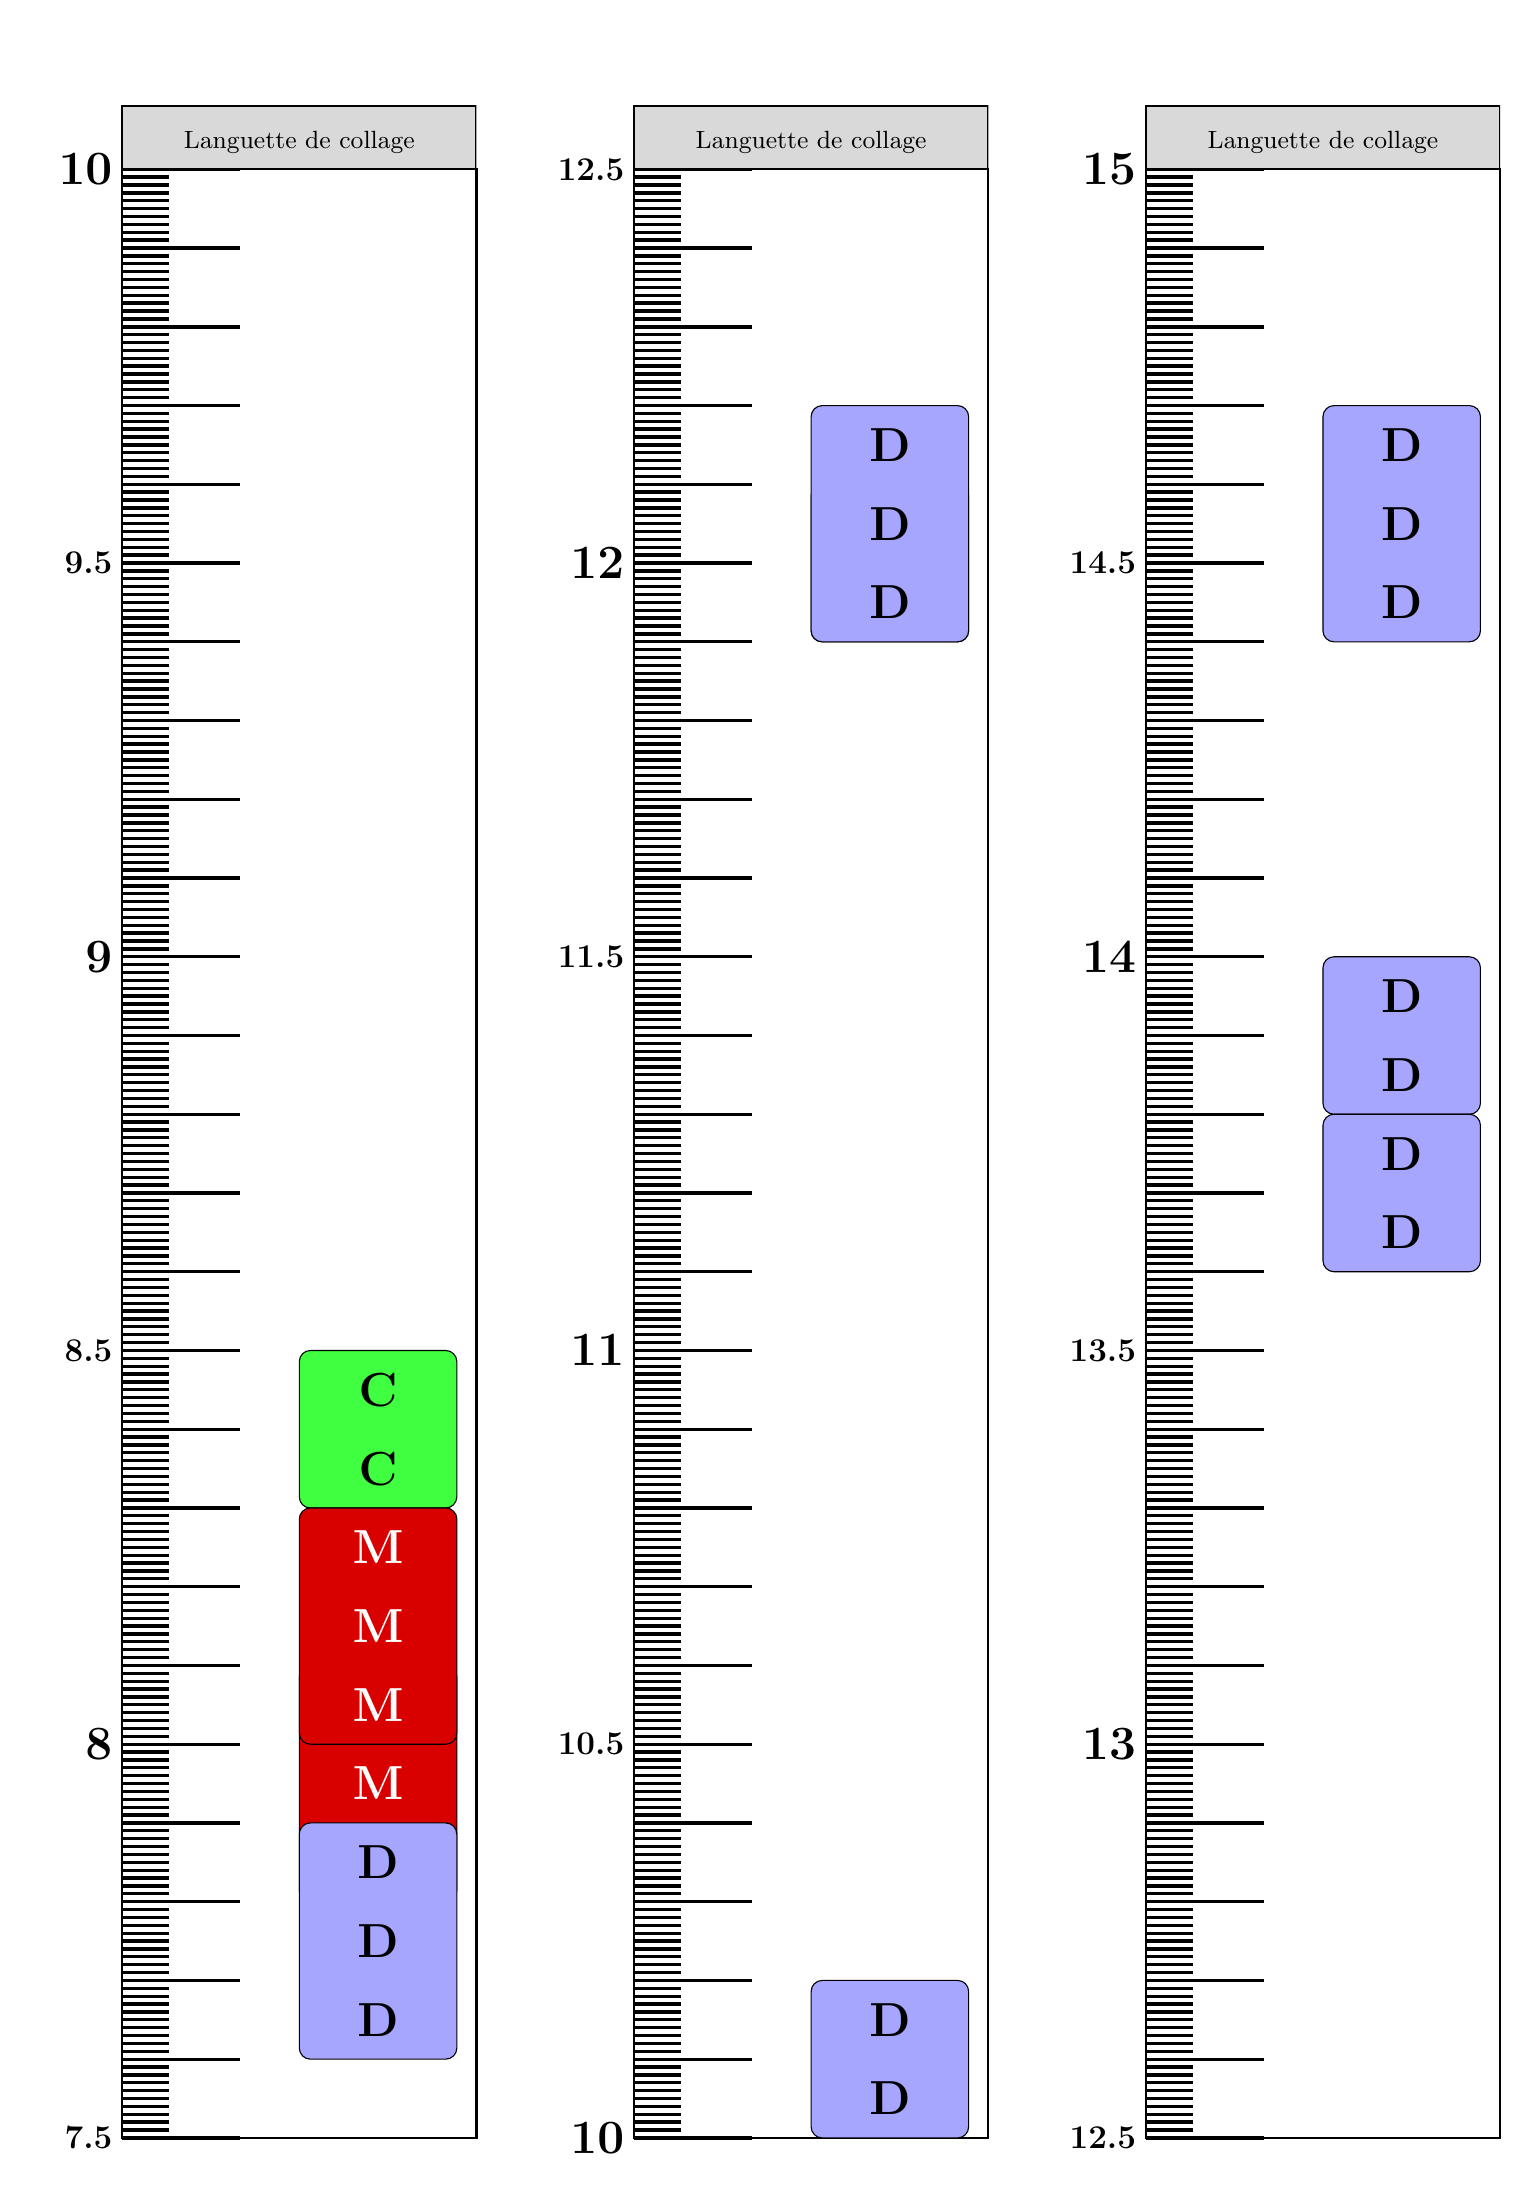
\begin{tikzpicture}[x=1cm, y=1cm,xshift=-1cm]
% Dessin de la première bande
\begin{scope}[shift={(-1,0)}]
    \draw[thick] (0,0) rectangle (\bandwidth, \bandheight);
    \clip (-1.2,-0.5) rectangle (\bandwidth, \bandheight+\languette+1);
    \drawGraduations{0}{25}{75}
\end{scope}

% Dessin de la deuxième bande (avec continuité des nombres)
\begin{scope}[shift={(1*\bandwidth + 1,0)}]
    \draw[thick] (0,0) rectangle (\bandwidth, \bandheight);
    \clip (-1.2,-0.5) rectangle (\bandwidth, \bandheight+\languette+1);
    \drawGraduations{0}{25}{100}
\end{scope}

% Dessin de la troisième bande (avec continuité des nombres)
\begin{scope}[shift={(2*\bandwidth + 3,0)}]
    \draw[thick] (0,0) rectangle (\bandwidth, \bandheight);
    \clip (-1.2,-0.5) rectangle (\bandwidth, \bandheight+\languette+1);
    \drawGraduations{0}{25}{125}
\end{scope}

\end{tikzpicture}

\newpage

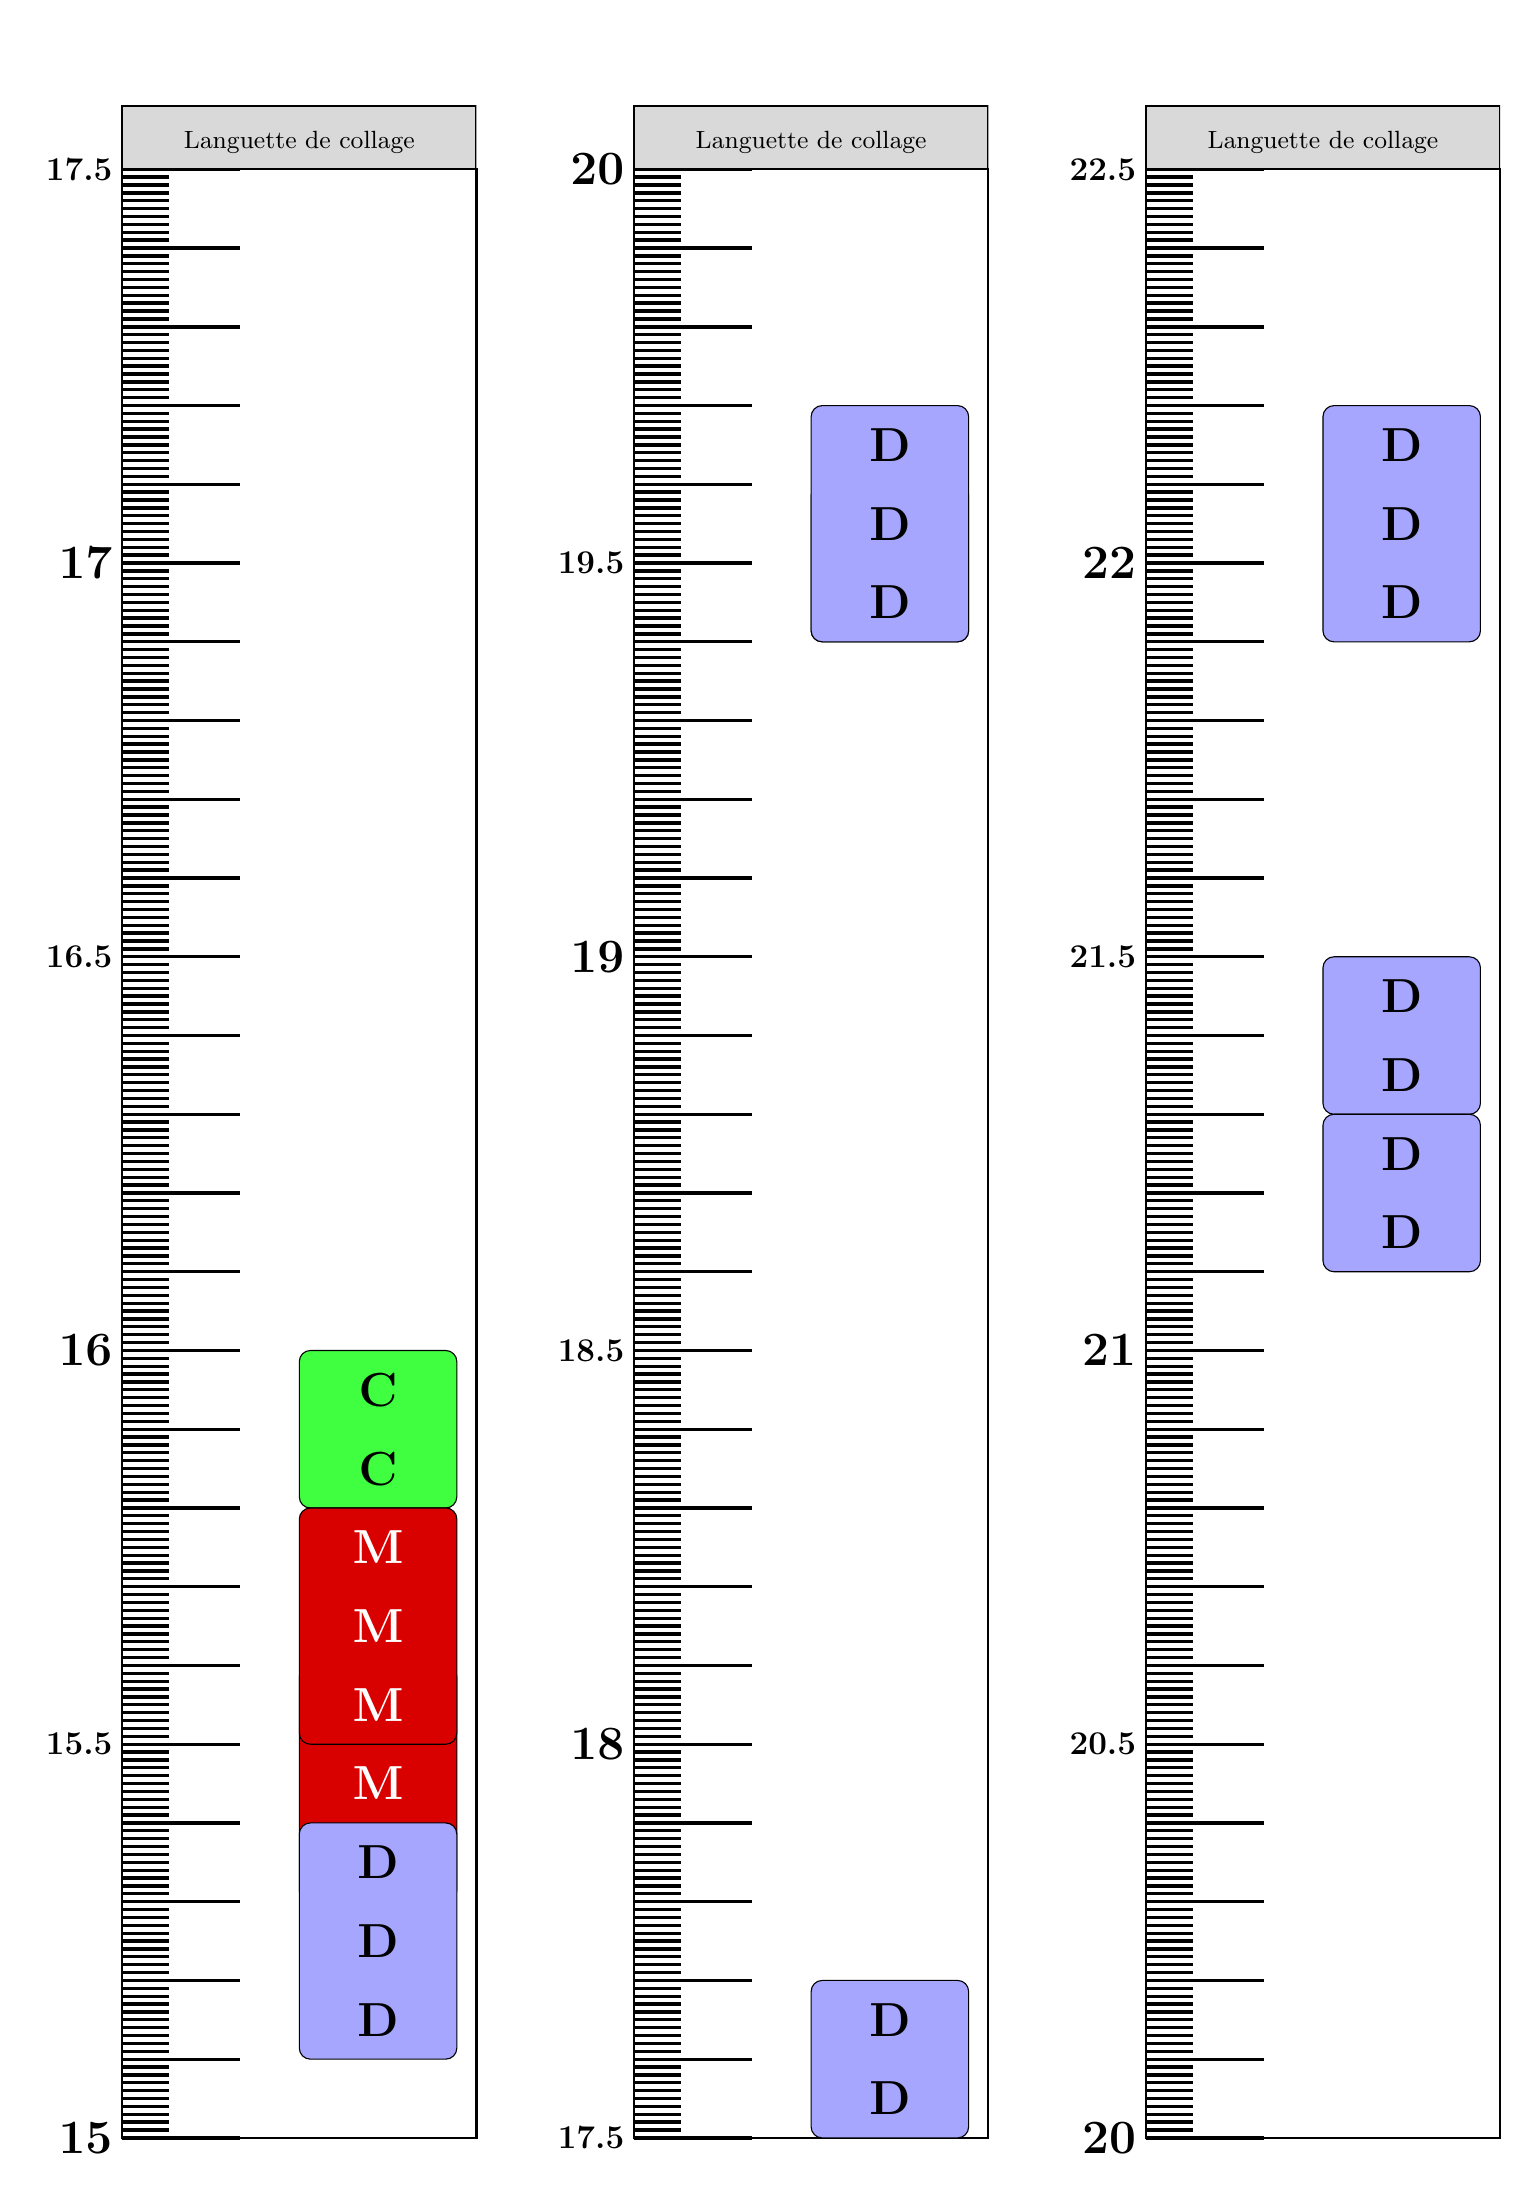
\begin{tikzpicture}[x=1cm, y=1cm,xshift=-1cm]
% Dessin de la première bande
\begin{scope}[shift={(-1,0)}]
    \draw[thick] (0,0) rectangle (\bandwidth, \bandheight);
    \clip (-1.2,-0.5) rectangle (\bandwidth, \bandheight+\languette+1);
    \drawGraduations{0}{25}{150}
\end{scope}

% Dessin de la deuxième bande (avec continuité des nombres)
\begin{scope}[shift={(1*\bandwidth + 1,0)}]
    \draw[thick] (0,0) rectangle (\bandwidth, \bandheight);
    \clip (-1.2,-0.5) rectangle (\bandwidth, \bandheight+\languette+1);
    \drawGraduations{0}{25}{175}
\end{scope}

% Dessin de la troisième bande (avec continuité des nombres)
\begin{scope}[shift={(2*\bandwidth + 3,0)}]
    \draw[thick] (0,0) rectangle (\bandwidth, \bandheight);
    \clip (-1.2,-0.5) rectangle (\bandwidth, \bandheight+\languette+1);
    \drawGraduations{0}{25}{200}
\end{scope}

\end{tikzpicture}

\newpage

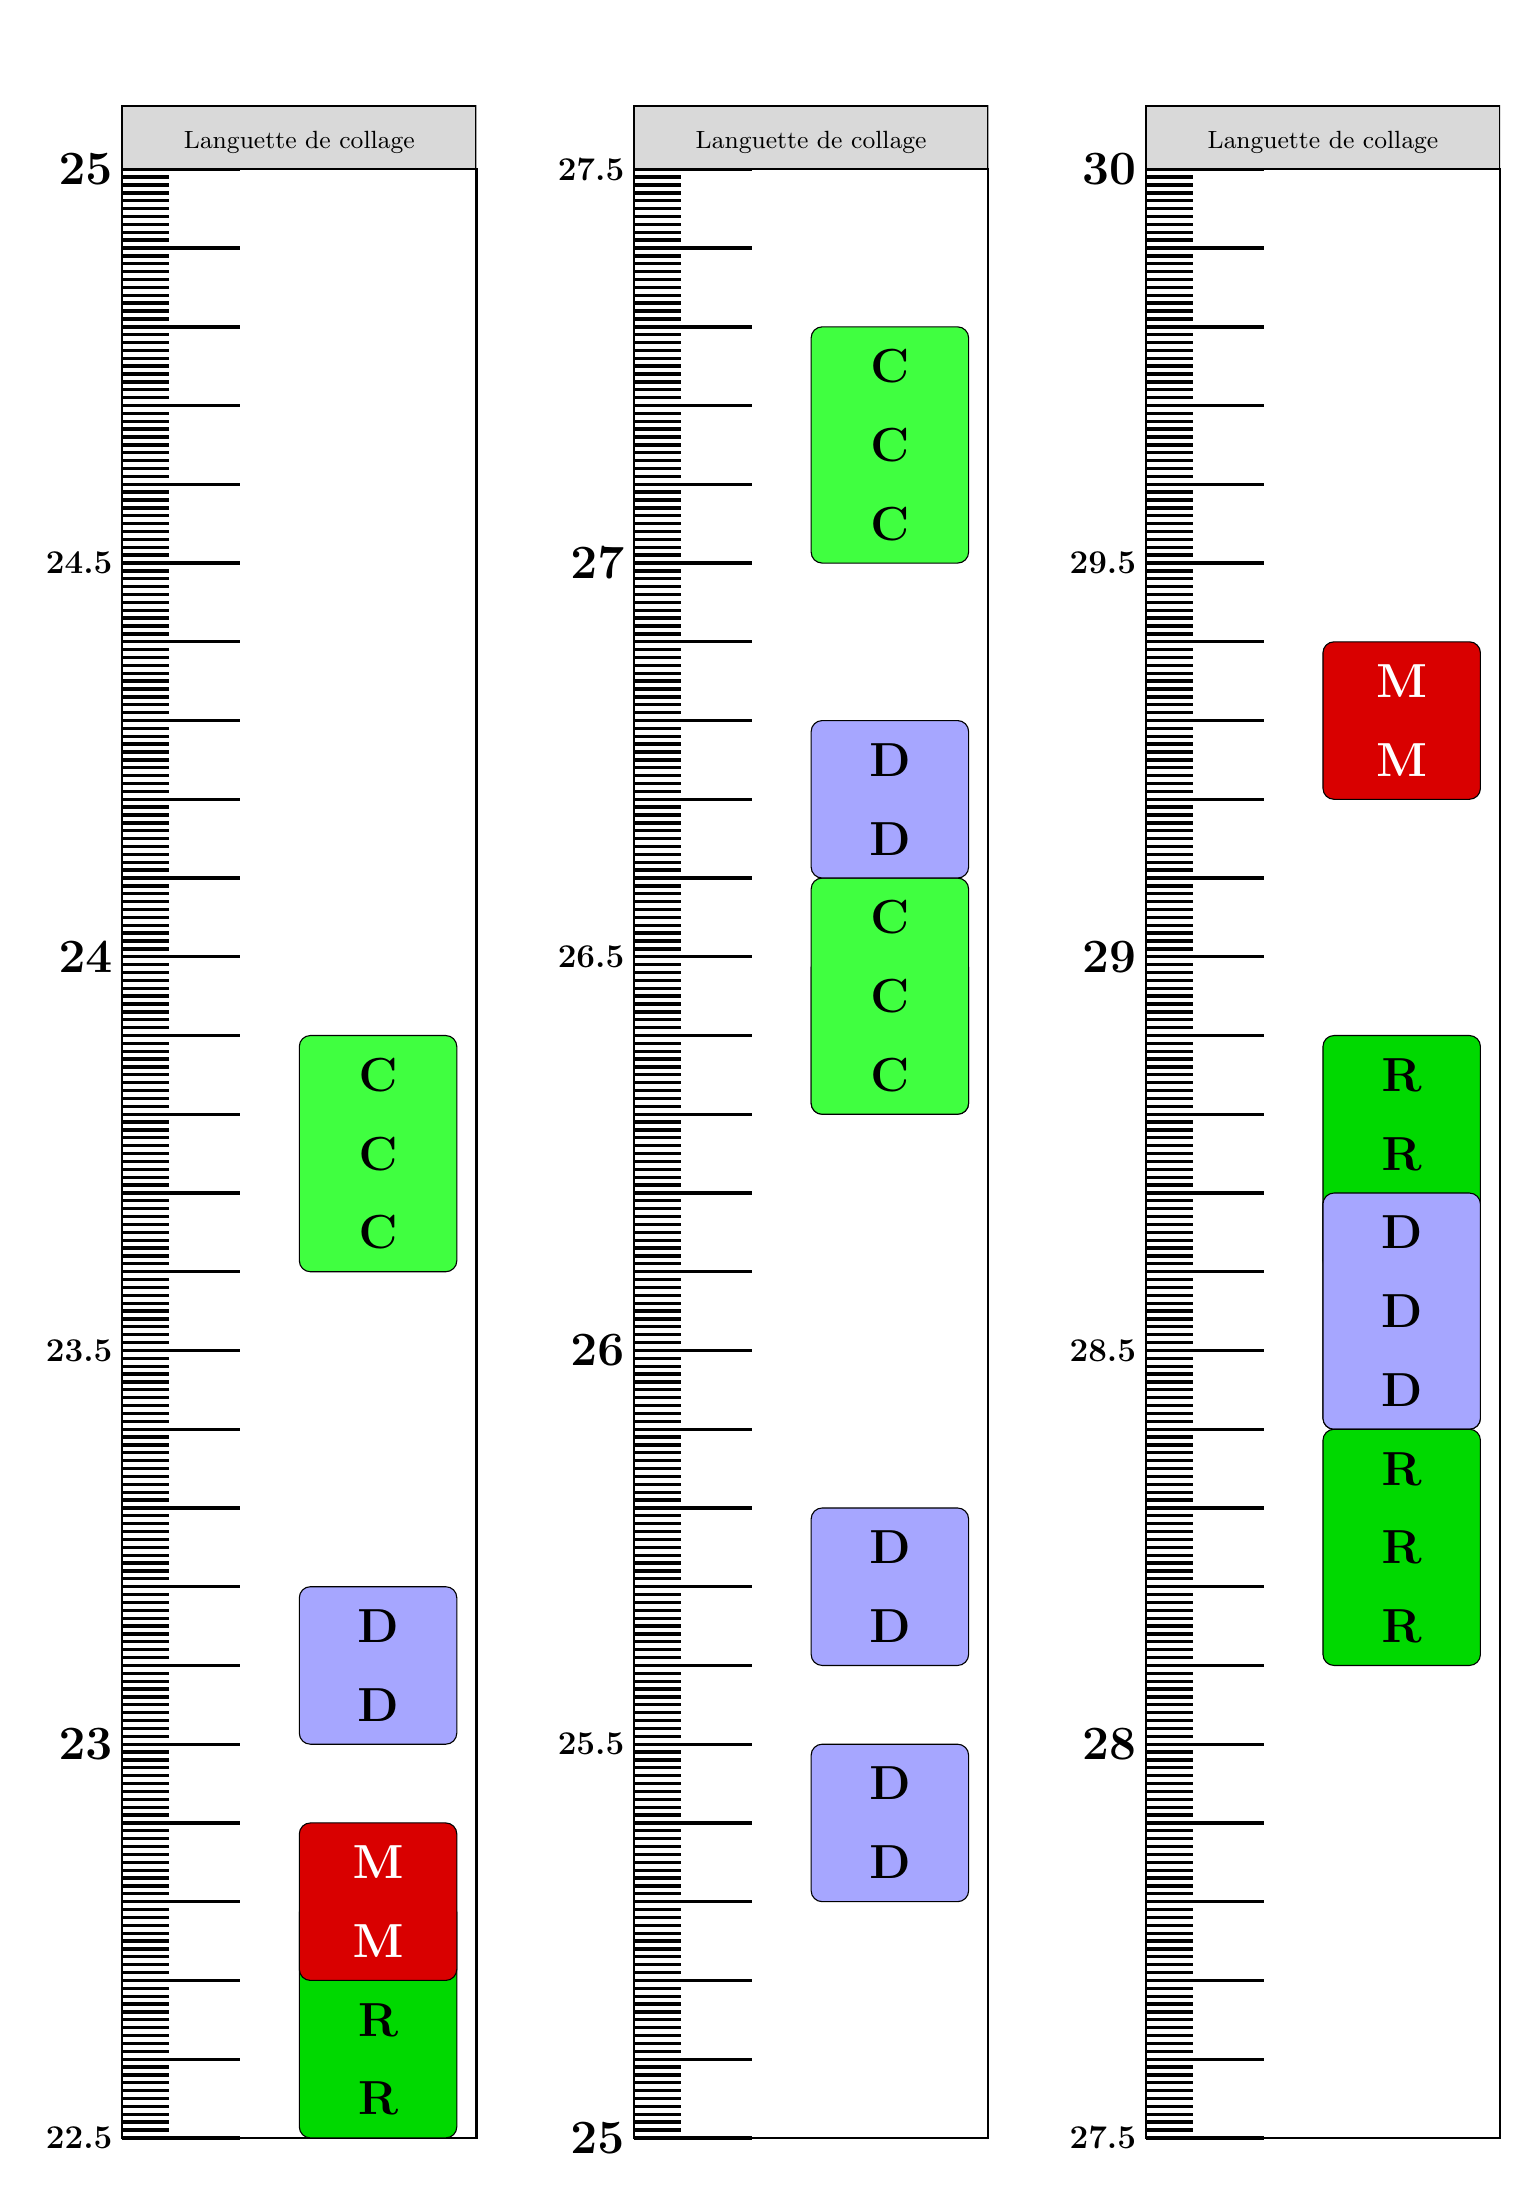
\begin{tikzpicture}[x=1cm, y=1cm,xshift=-1cm]
% Dessin de la première bande
\begin{scope}[shift={(-1,0)}]
    \draw[thick] (0,0) rectangle (\bandwidth, \bandheight);
    \clip (-1.2,-0.5) rectangle (\bandwidth, \bandheight+\languette+1);
    \drawGraduations{0}{25}{225}
\end{scope}

% Dessin de la deuxième bande (avec continuité des nombres)
\begin{scope}[shift={(1*\bandwidth + 1,0)}]
    \draw[thick] (0,0) rectangle (\bandwidth, \bandheight);
    \clip (-1.2,-0.5) rectangle (\bandwidth, \bandheight+\languette+1);
    \drawGraduations{0}{25}{250}
\end{scope}

% Dessin de la troisième bande (avec continuité des nombres)
\begin{scope}[shift={(2*\bandwidth + 3,0)}]
    \draw[thick] (0,0) rectangle (\bandwidth, \bandheight);
    \clip (-1.2,-0.5) rectangle (\bandwidth, \bandheight+\languette+1);
    \drawGraduations{0}{25}{275}
\end{scope}

\end{tikzpicture}

\newpage

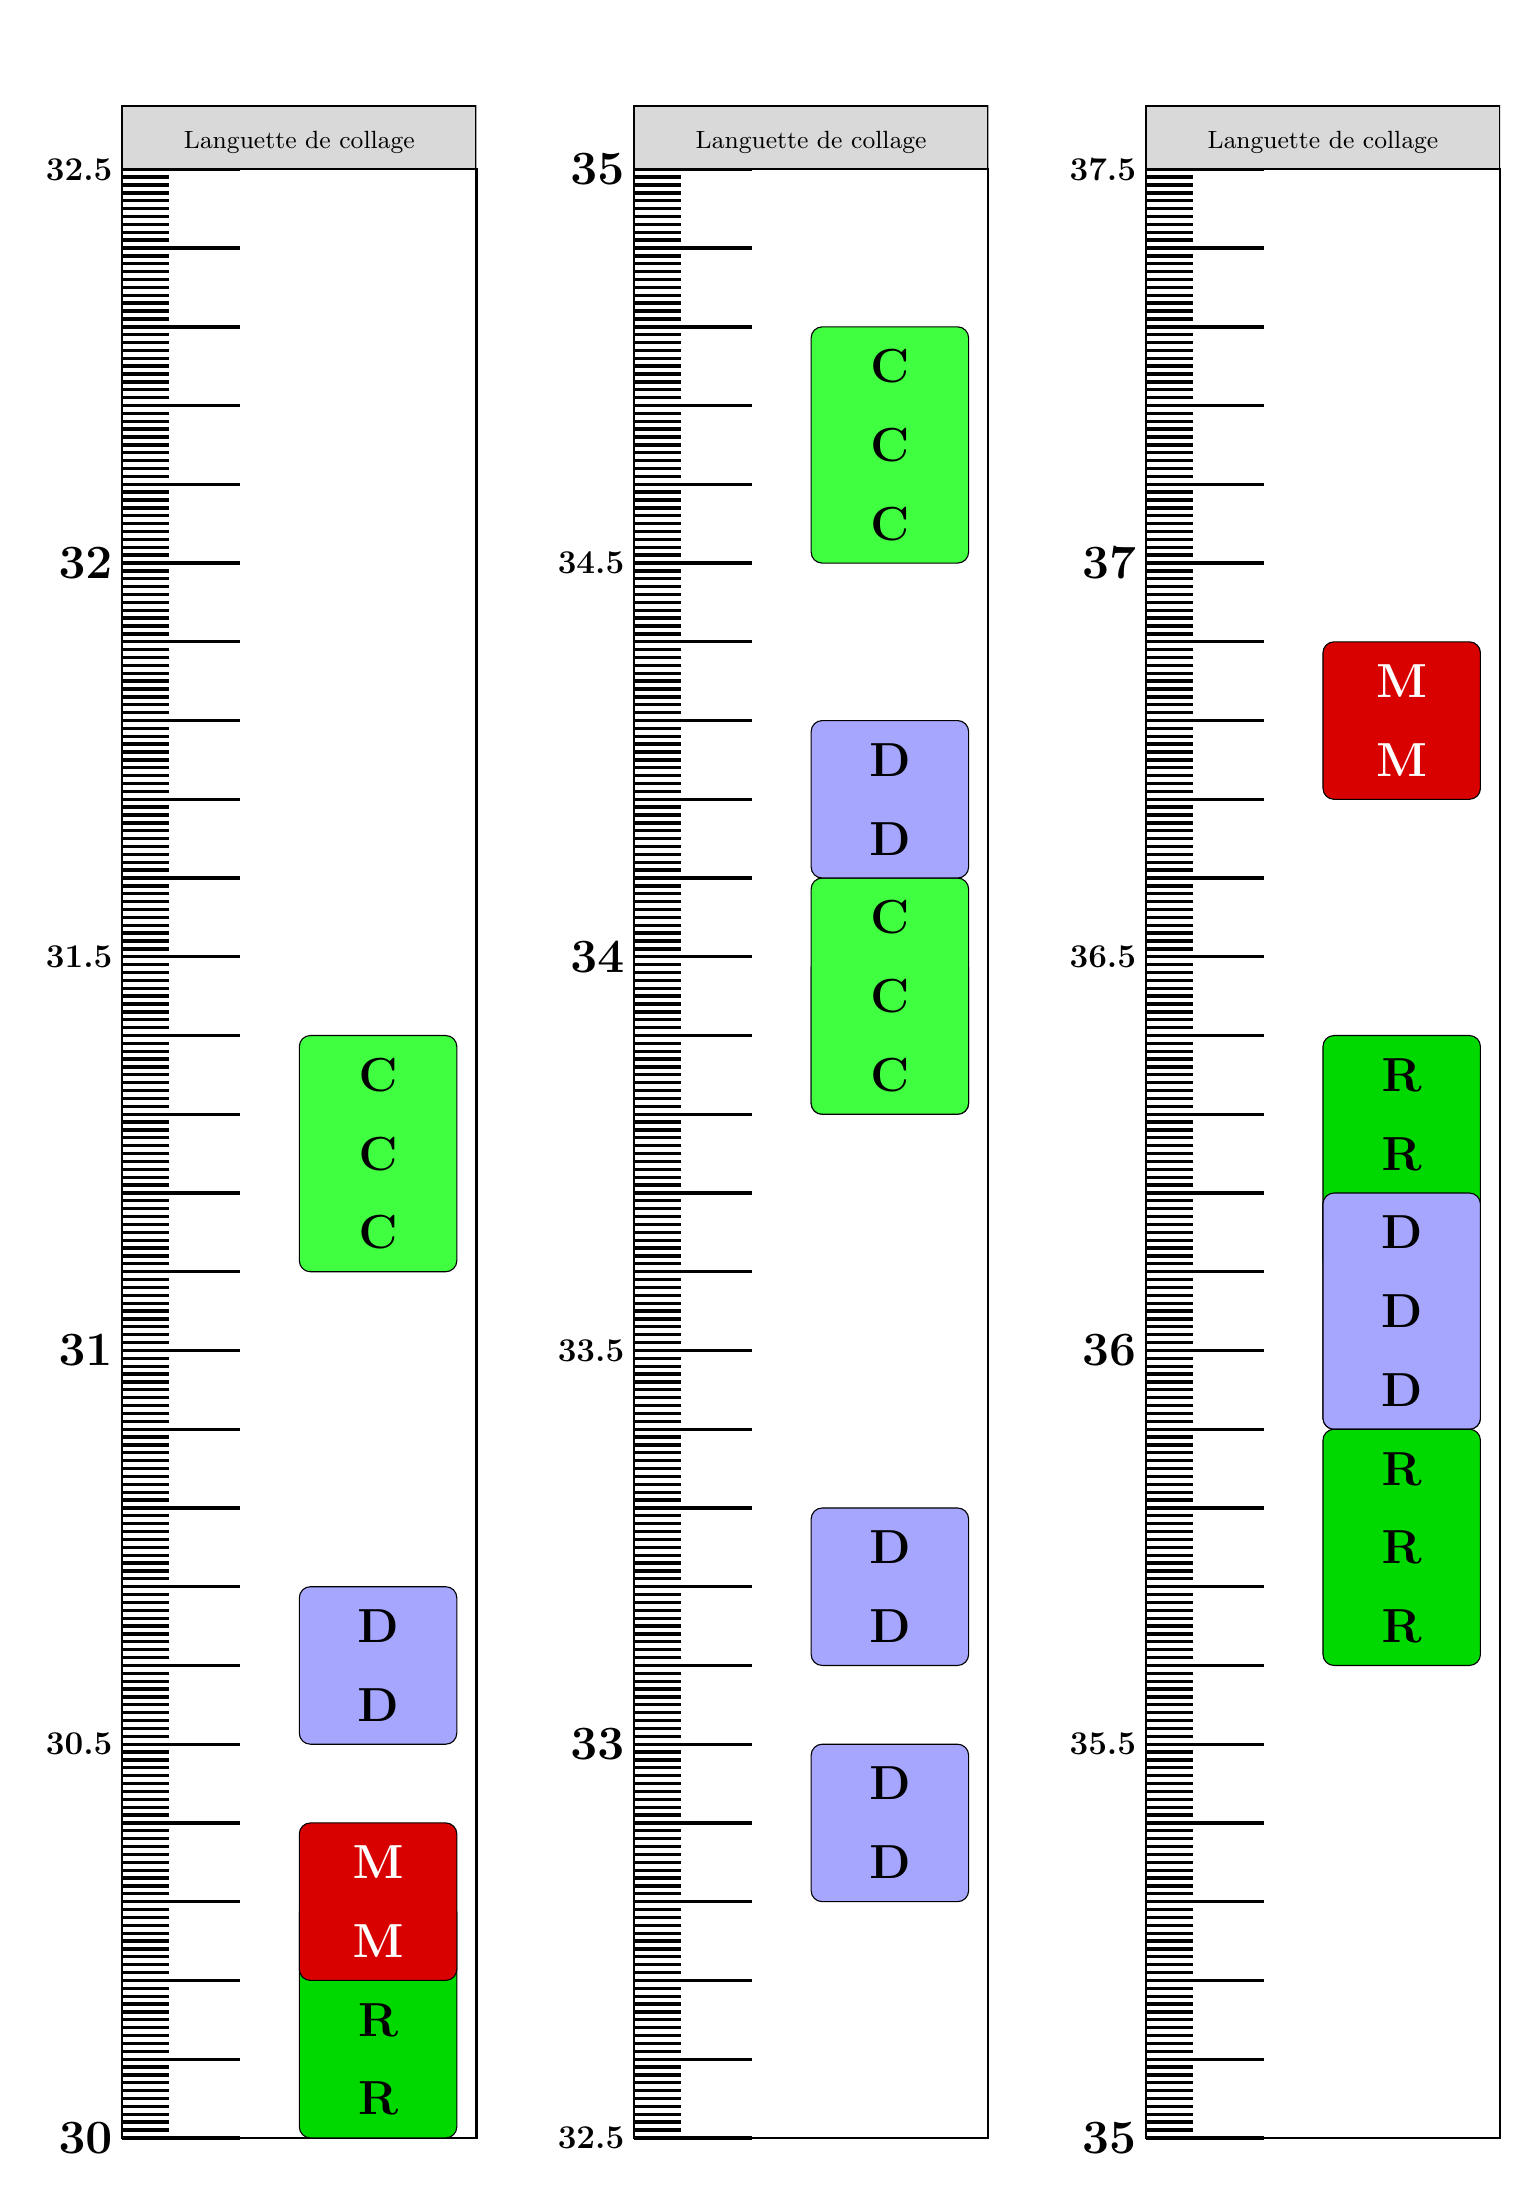
\begin{tikzpicture}[x=1cm, y=1cm,xshift=-1cm]
% Dessin de la première bande
\begin{scope}[shift={(-1,0)}]
    \draw[thick] (0,0) rectangle (\bandwidth, \bandheight);
    \clip (-1.2,-0.5) rectangle (\bandwidth, \bandheight+\languette+1);
    \drawGraduations{0}{25}{300}
\end{scope}

% Dessin de la deuxième bande (avec continuité des nombres)
\begin{scope}[shift={(1*\bandwidth + 1,0)}]
    \draw[thick] (0,0) rectangle (\bandwidth, \bandheight);
    \clip (-1.2,-0.5) rectangle (\bandwidth, \bandheight+\languette+1);
    \drawGraduations{0}{25}{325}
\end{scope}

% Dessin de la troisième bande (avec continuité des nombres)
\begin{scope}[shift={(2*\bandwidth + 3,0)}]
    \draw[thick] (0,0) rectangle (\bandwidth, \bandheight);
    \clip (-1.2,-0.5) rectangle (\bandwidth, \bandheight+\languette+1);
    \drawGraduations{0}{25}{350}
\end{scope}

\end{tikzpicture}

\newpage

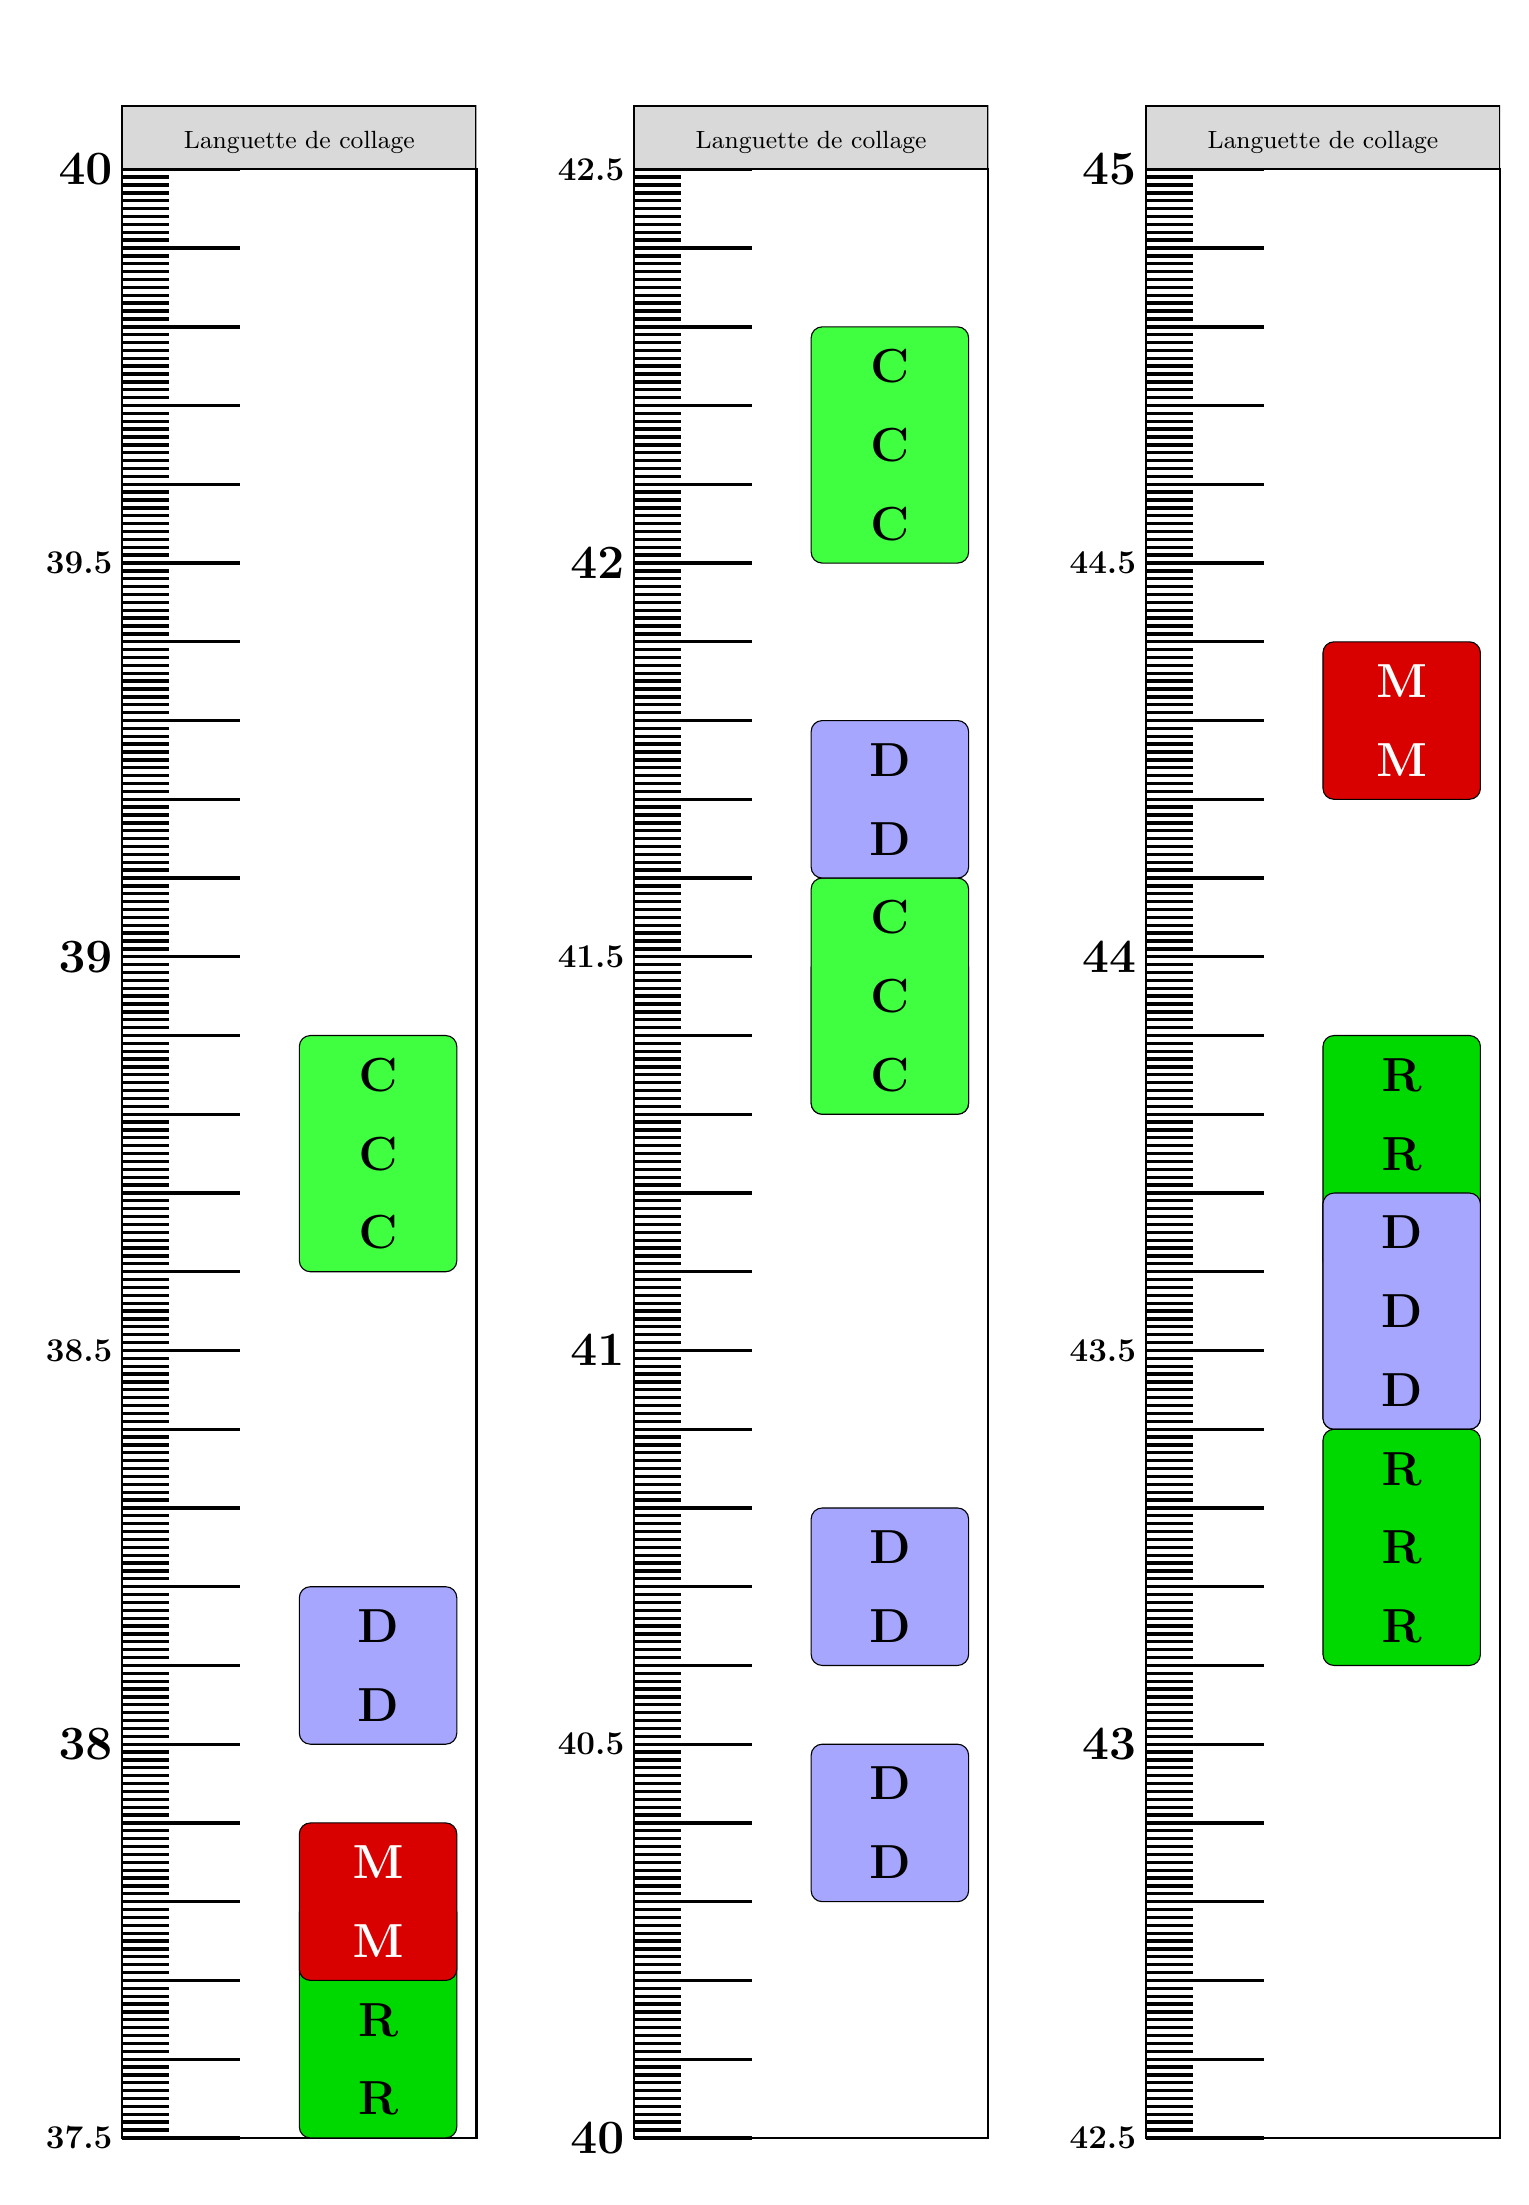
\begin{tikzpicture}[x=1cm, y=1cm,xshift=-1cm]
% Dessin de la première bande
\begin{scope}[shift={(-1,0)}]
    \draw[thick] (0,0) rectangle (\bandwidth, \bandheight);
    \clip (-1.2,-0.5) rectangle (\bandwidth, \bandheight+\languette+1);
    \drawGraduations{0}{25}{375}
\end{scope}

% Dessin de la deuxième bande (avec continuité des nombres)
\begin{scope}[shift={(1*\bandwidth + 1,0)}]
    \draw[thick] (0,0) rectangle (\bandwidth, \bandheight);
    \clip (-1.2,-0.5) rectangle (\bandwidth, \bandheight+\languette+1);
    \drawGraduations{0}{25}{400}
\end{scope}

% Dessin de la troisième bande (avec continuité des nombres)
\begin{scope}[shift={(2*\bandwidth + 3,0)}]
    \draw[thick] (0,0) rectangle (\bandwidth, \bandheight);
    \clip (-1.2,-0.5) rectangle (\bandwidth, \bandheight+\languette+1);
    \drawGraduations{0}{25}{425}
\end{scope}

\end{tikzpicture}

\newpage

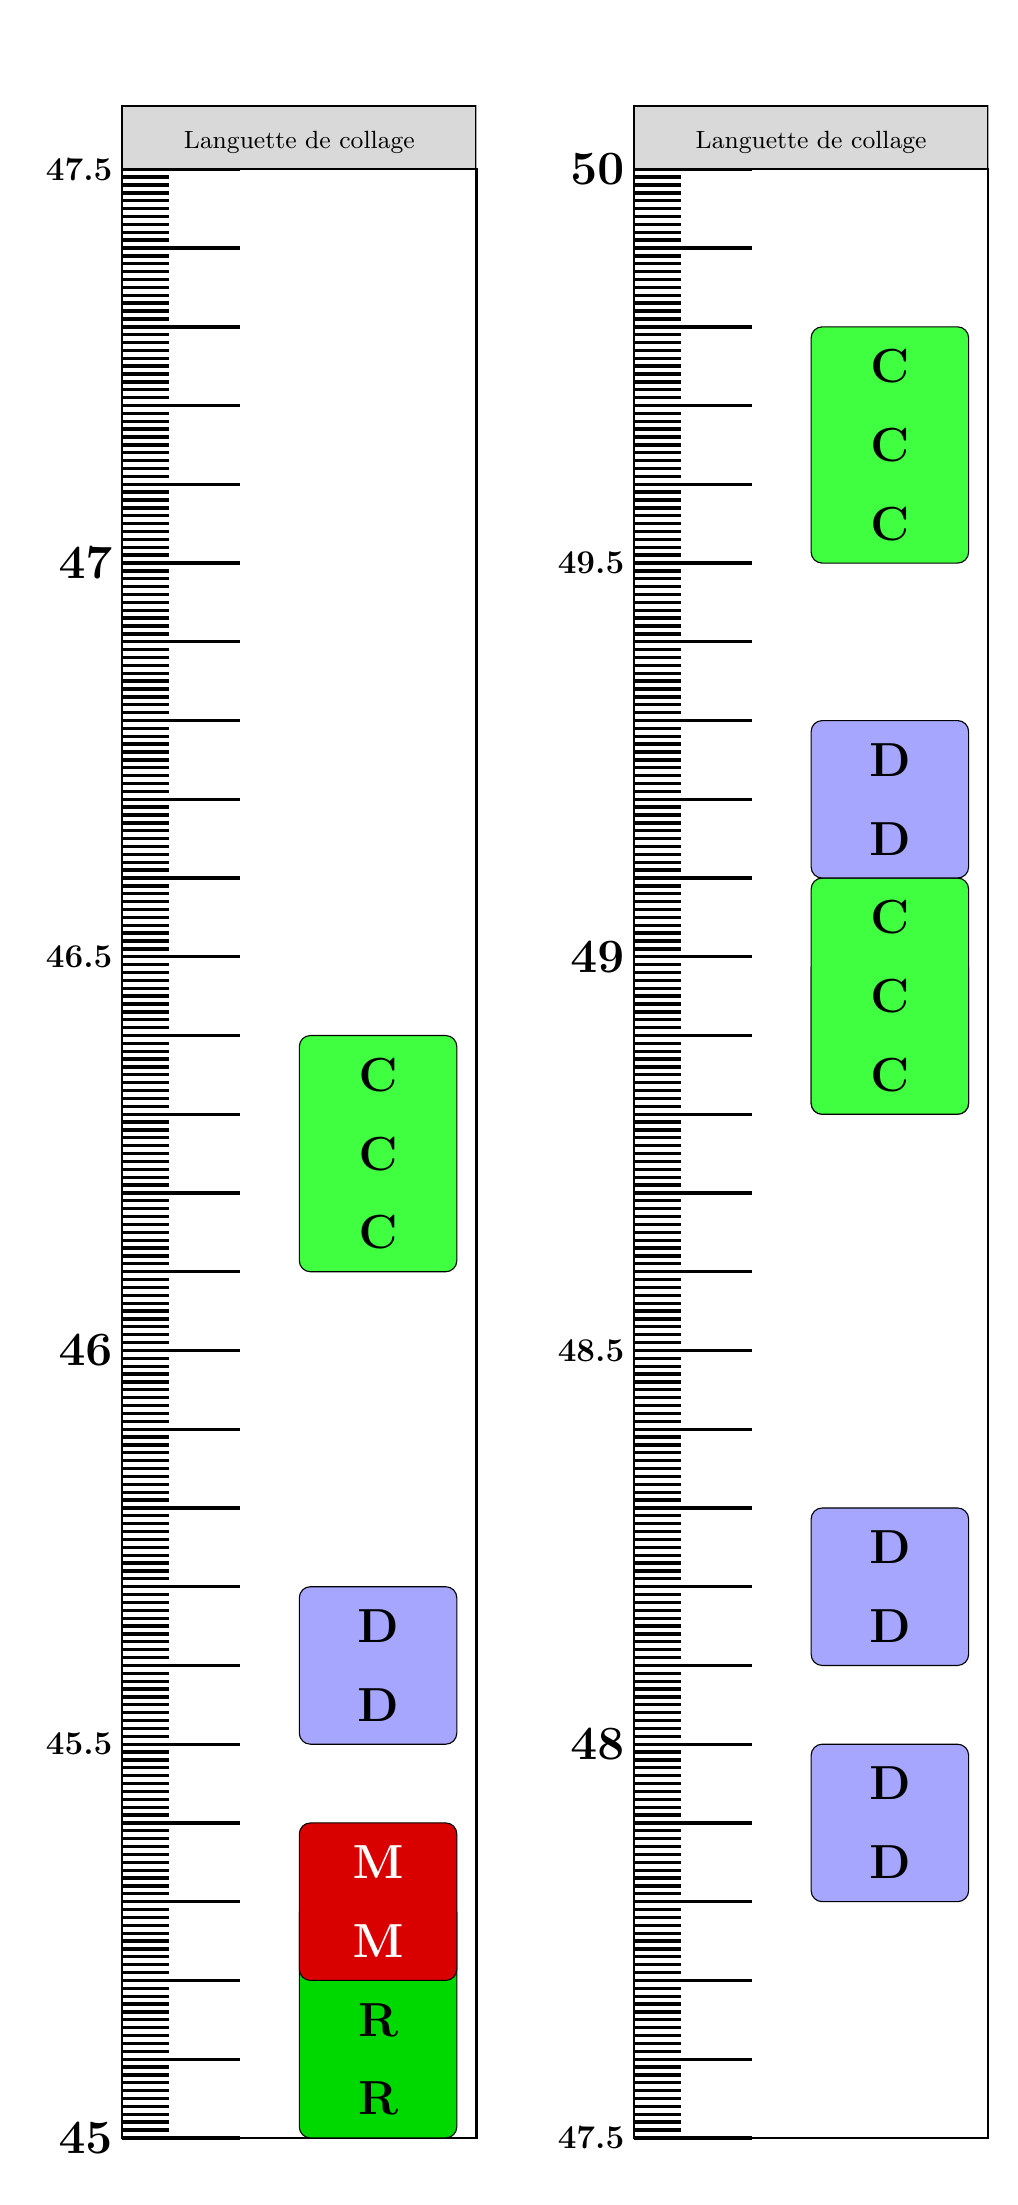
\begin{tikzpicture}[x=1cm, y=1cm,xshift=-1cm]
% Dessin de la première bande
\begin{scope}[shift={(-1,0)}]
    \draw[thick] (0,0) rectangle (\bandwidth, \bandheight);
    \clip (-1.2,-0.5) rectangle (\bandwidth, \bandheight+\languette+1);
    \drawGraduations{0}{25}{450}
\end{scope}

% Dessin de la deuxième bande (avec continuité des nombres)
\begin{scope}[shift={(1*\bandwidth + 1,0)}]
    \draw[thick] (0,0) rectangle (\bandwidth, \bandheight);
    \clip (-1.2,-0.5) rectangle (\bandwidth, \bandheight+\languette+1);
    \drawGraduations{0}{25}{475}
\end{scope}

\end{tikzpicture}


%\newpage

%\section{La grande frise}

%\renewcommand{\drawGraduations}[4]{%
    % #1: Start value
    % #2: End value
    % #3: Offset value (for continuity)

    % Centièmes graduations (réduction du nombre de graduations)
    \def\scalefactor{2}

    \foreach \x in {#1,0.1,...,#2} {
        \draw[very thick] (0,\x*\scalefactor) -- (0.6, \x*\scalefactor);
    }

    % Dixièmes graduations
    \foreach \x in {\fpeval{#1},1,...,#2} {
        \draw[very thick] (0,\fpeval{(\x+#4)*\scalefactor}) -- (1.5, \fpeval{(\x+#4)*\scalefactor});
    }

    % Unités graduations et affichage en grand et gras pour les entiers
    \foreach \x in {\fpeval{#1+#4},1,...,\fpeval{#2+0.1}} {
        \pgfmathsetmacro{\write}{(\x + #3) / (10)}
        \pgfmathsetmacro{\value}{((\x + #3)*\scalefactor) / (10)}
        \pgfmathsetmacro{\semivalue}{((\x + #3 + 5*#4)*\scalefactor)  / (10)}
        \pgfmathsetmacro{\semiremainder}{mod(\semivalue,1)}
        \pgfmathsetmacro{\remainder}{mod(\value,1)}
        \ifdim \remainder pt = 0pt
            \node[left, font=\bfseries\LARGE] at (0, \x*\scalefactor) {\num{\fpeval{\write}}};
            %\draw[very thick] (0,\x*\scalefactor+#4) -- (1.5, \x*\scalefactor+#4);
        \fi
        %\ifdim \semiremainder pt = 0pt
        %    \node[left, font=\bfseries\large] at (0, \x*\scalefactor) {\num{\fpeval{\write}}};
        %    %\draw[very thick] (0,\x*\scalefactor+#4) -- (1.5, \x*\scalefactor+#4);
        %\fi
    }

        % Gamification : ajouter des événements aléatoires
        \pgfmathsetmacro{\randomShift}{rnd*4 - 2} % Générer une variation entre -2 et +2
        \pgfmathsetmacro{\eventCount}{int(\fpeval{(5 + \randomShift)/\scalefactor})} % Base 5 événements avec une variation de -2 à +2
        \foreach \i in {1,...,\eventCount} {
        \pgfmathsetmacro{\randY}{random(\fpeval{#1*\scalefactor},\fpeval{(#2 - 3)*\scalefactor})}
        \pgfmathrandominteger{\randheight}{1}{2}
        \pgfmathsetmacro{\randX}{0.5*\bandwidth}
        \pgfmathrandominteger{\eventType}{1}{4}
        \def\eventcolor{yellow}
        \def\eventTextColor{black}
        % Définition des labels selon l'événement
        \ifnum\eventType=1
            \def\eventText{R}%Relancer les dés
            \def\eventcolor{green!85!black}
        \fi
        \ifnum\eventType=2
            \def\eventText{M}%Événement malchanceux}
            \def\eventcolor{red!85!black}
            \def\eventTextColor{white}
        \fi
        \ifnum\eventType=3
            \def\eventText{C}%Événement chanceux}
            \def\eventcolor{green!75!white}
        \fi
        \ifnum\eventType=4
            \def\eventText{D}%Défi}
            \def\eventcolor{orange}
        \fi
        % Dessiner l'événement à une position aléatoire
        \draw[fill=\eventcolor, rounded corners] (\randX, \randY) rectangle ++(2, \fpeval{(\randheight+1)*\scalefactor});

        % Calcul de l'intervalle et placement des labels
        \pgfmathsetmacro{\startY}{\randY}
        \pgfmathsetmacro{\endY}{\randY + \randheight*\scalefactor}
        \foreach \y in {\startY, \fpeval{\startY + 1*\scalefactor}, ..., \endY} {
            \node at (\randX + 1, \y + 0.5*\scalefactor) {\LARGE{\textbf{\color{\eventTextColor}\eventText}}};
        }
    }
    
    % Languette de collage pour lier à la frise suivante
    \draw[thick, fill=gray!30] (0, \bandheight) rectangle (\bandwidth, \bandheight + \languette);
    \node[above, font=\small] at (\bandwidth/2, \bandheight + \languette / 10) {Languette de collage};
}

La frise suivante est à découper. 

Il suffit ensuite de coller les languettes, pour assembler la frise.

\def\scalefactor{2}
Longueur totale : $\num{\fpeval{10 * \scalefactor * 137.5}}$
\newpage

% Définition des constantes
\def\bandwidth{4.5} % Largeur d'une bande en cm
\def\bandheight{25} % Hauteur d'une bande en cm
\def\languette{0.8}
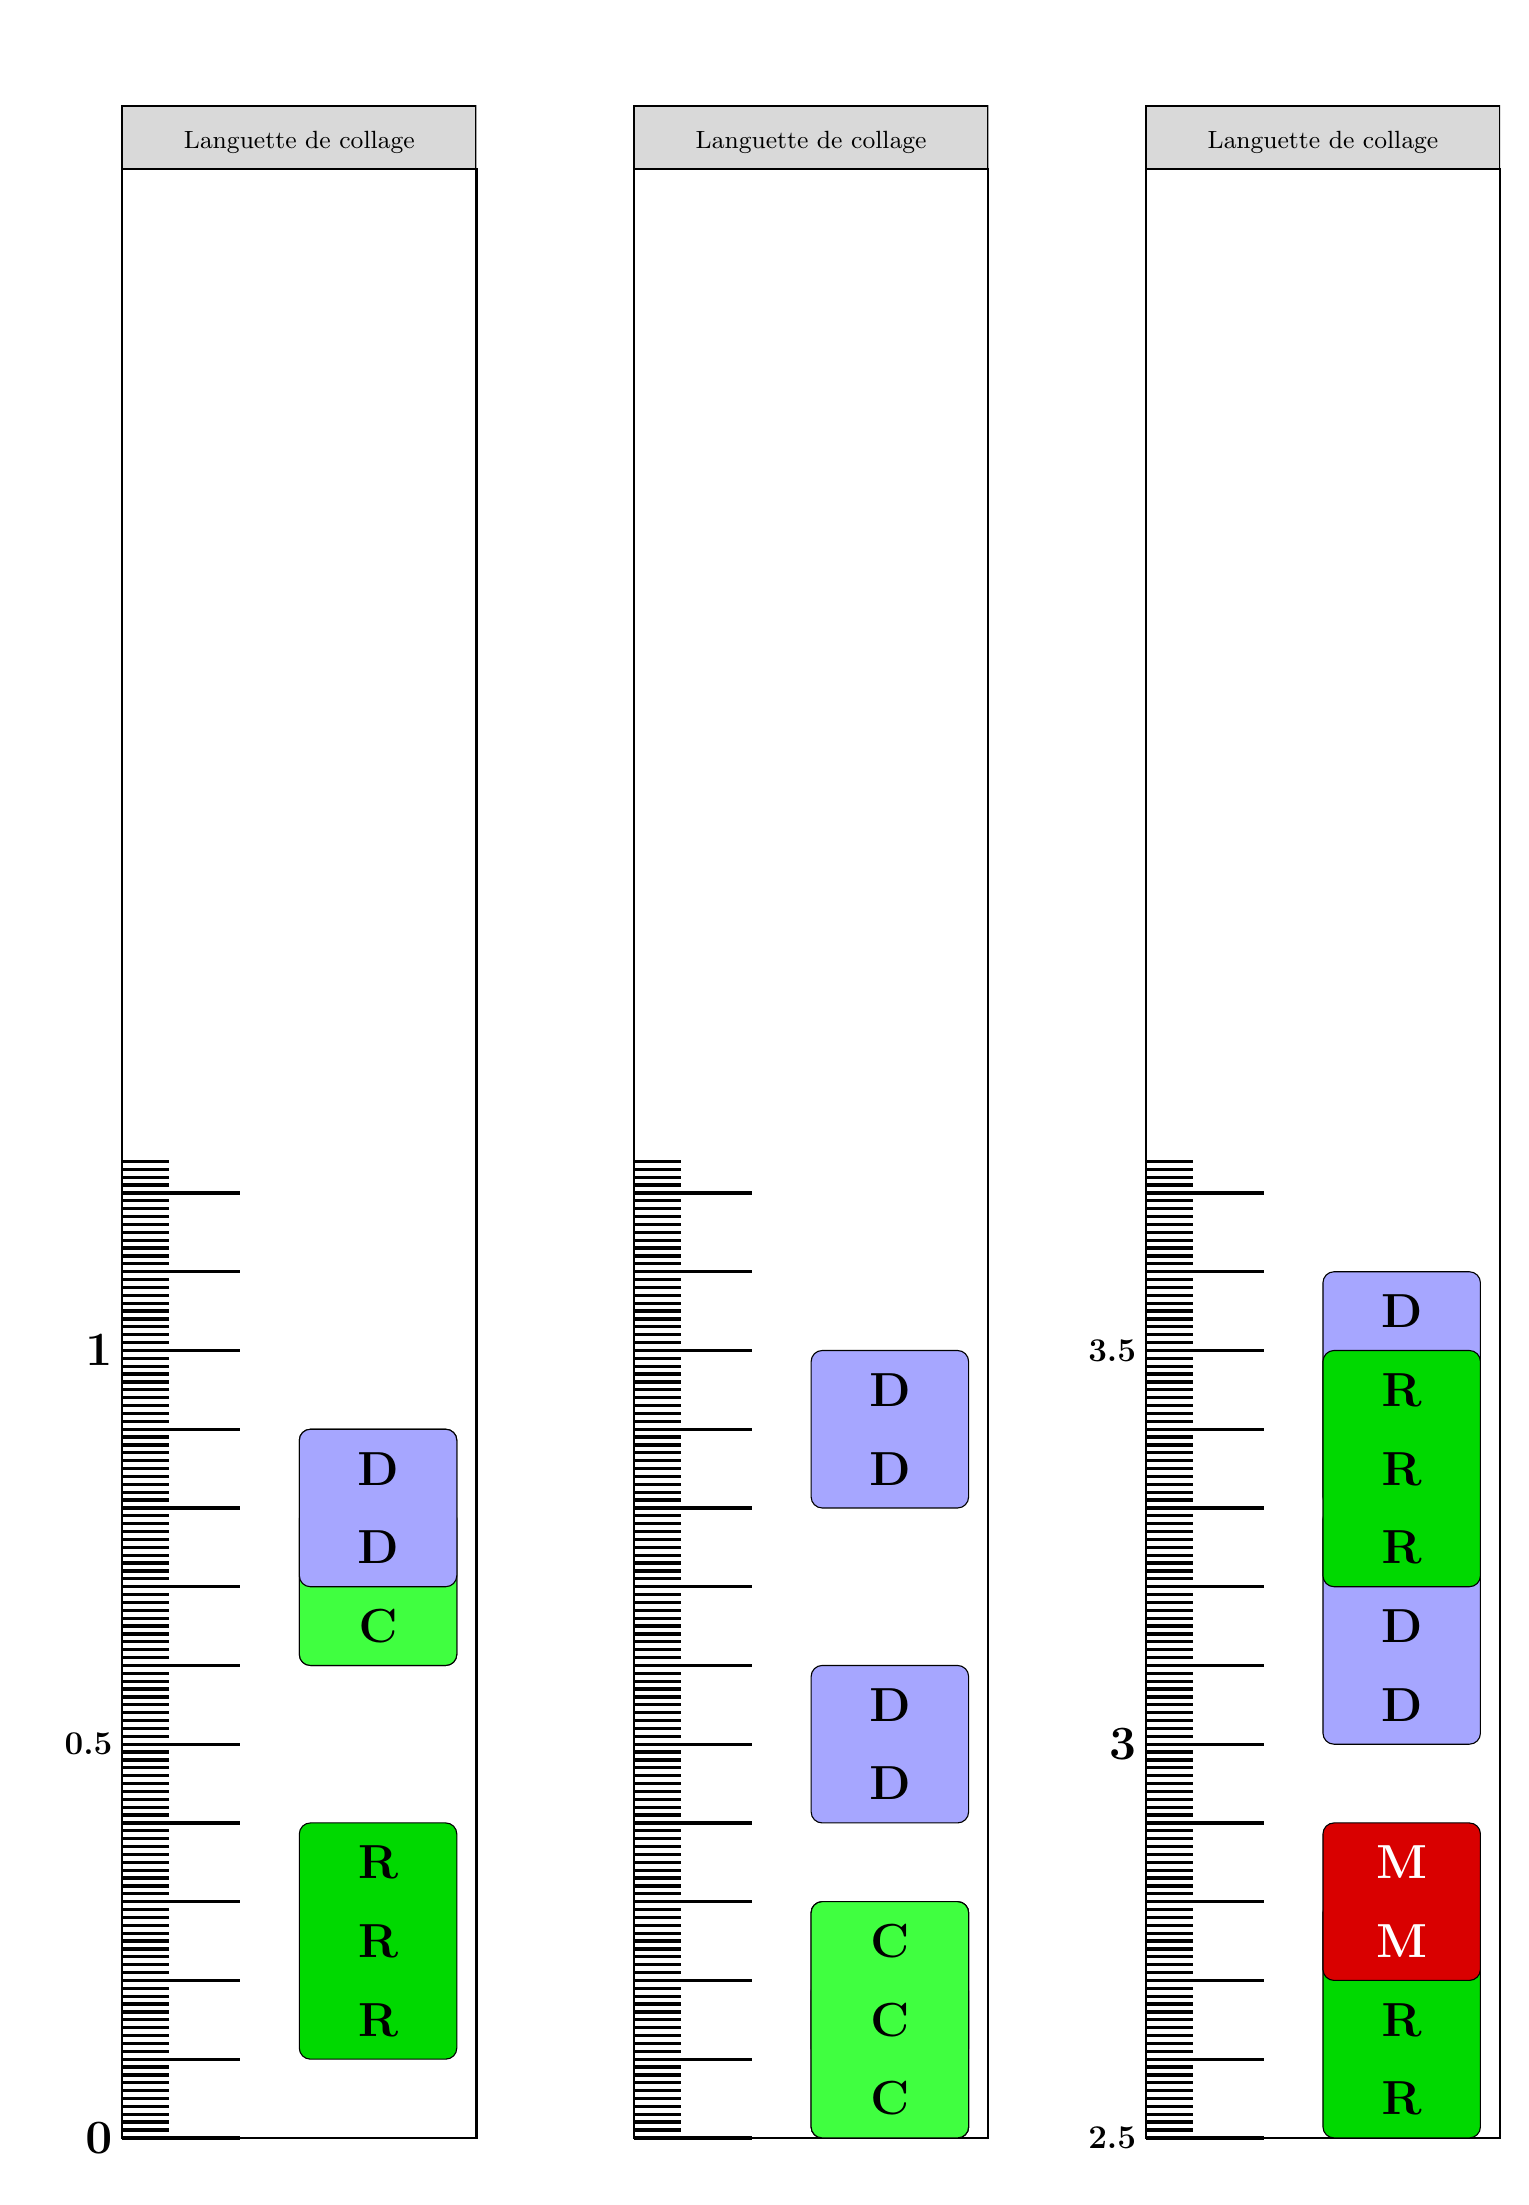
\begin{tikzpicture}[x=1cm, y=1cm,xshift=-1cm]

% Dessin de la première bande
\begin{scope}[shift={(-1,0)}]
    \draw[thick] (0,0) rectangle (\bandwidth, \bandheight);
    \clip (-1.2,-0.5) rectangle (\bandwidth, \bandheight+\languette+1);
    \drawGraduations{0}{12.5}{0}{0}
\end{scope}

% Dessin de la deuxième bande (avec continuité des nombres)
\begin{scope}[shift={(1*\bandwidth + 1,0)}]
    \draw[thick] (0,0) rectangle (\bandwidth, \bandheight);
    \clip (-1.2,-0.5) rectangle (\bandwidth, \bandheight+\languette+1);
    \drawGraduations{0}{12.5}{12.5}{0.5}
\end{scope}

% Dessin de la troisième bande (avec continuité des nombres)
\begin{scope}[shift={(2*\bandwidth + 3,0)}]
    \draw[thick] (0,0) rectangle (\bandwidth, \bandheight);
    \clip (-1.2,-0.5) rectangle (\bandwidth, \bandheight+\languette+1);
    \drawGraduations{0}{12.5}{25}{0}
\end{scope}

\end{tikzpicture}

\newpage

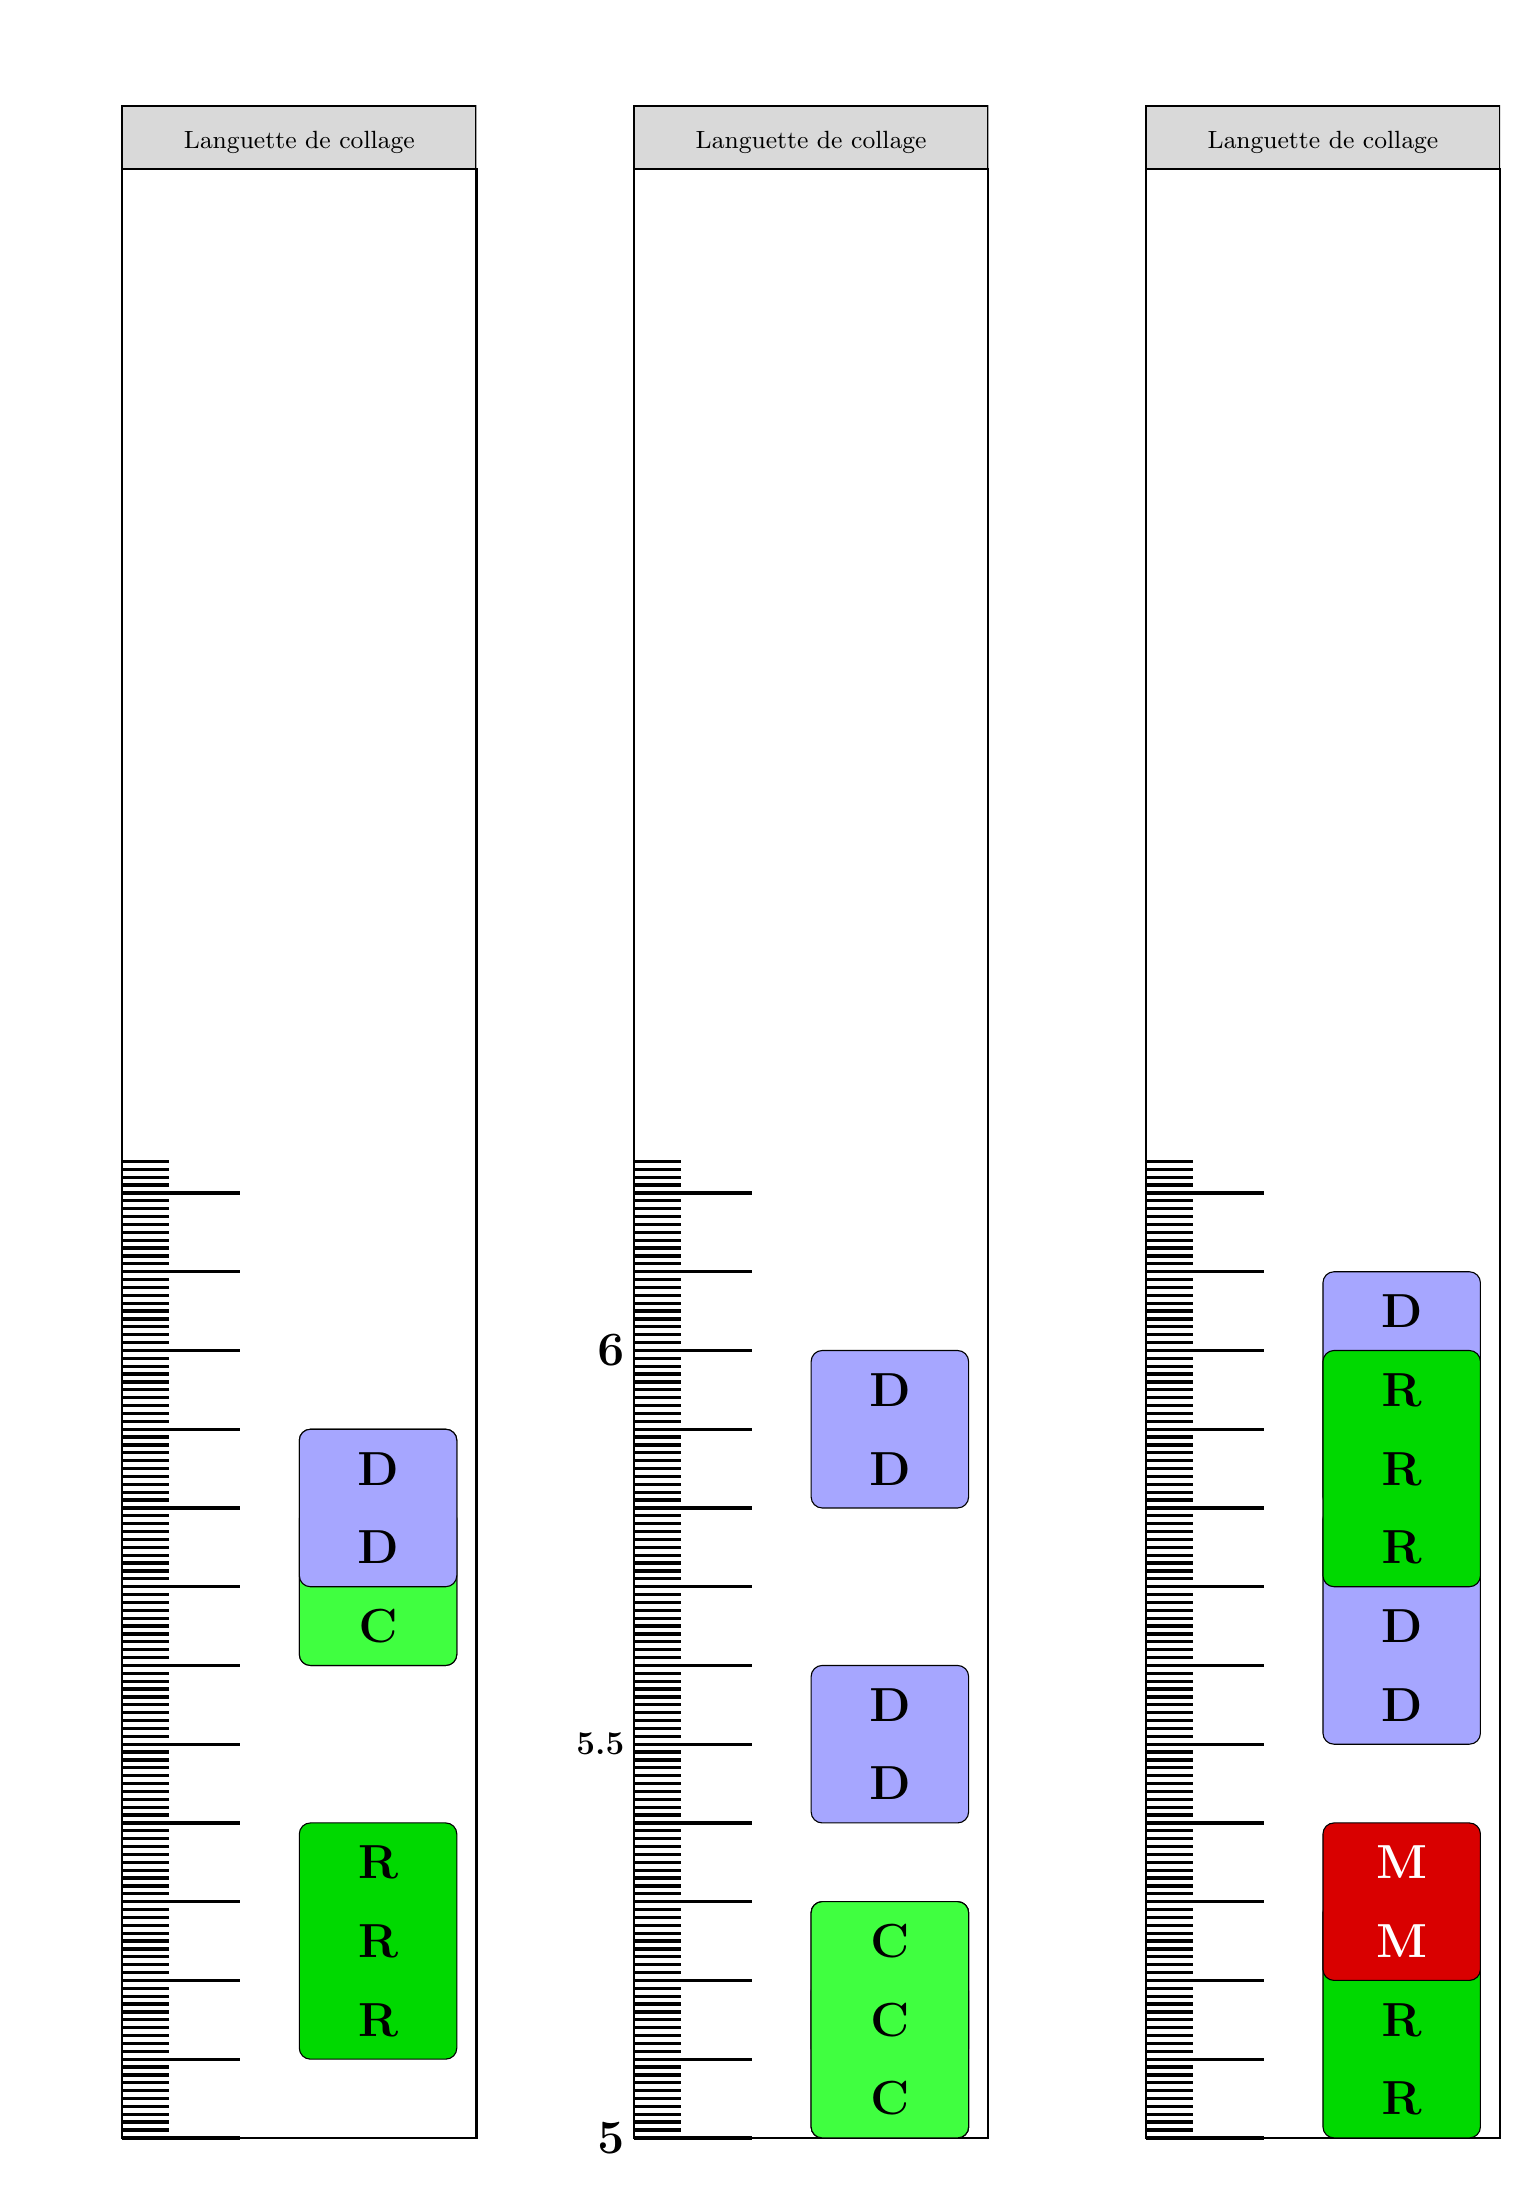
\begin{tikzpicture}[x=1cm, y=1cm,xshift=-1cm]
% Dessin de la première bande
\begin{scope}[shift={(-1,0)}]
    \draw[thick] (0,0) rectangle (\bandwidth, \bandheight);
    \clip (-1.2,-0.5) rectangle (\bandwidth, \bandheight+\languette+1);
    \drawGraduations{0}{12.5}{37.5}{0.5}
\end{scope}

% Dessin de la deuxième bande (avec continuité des nombres)
\begin{scope}[shift={(1*\bandwidth + 1,0)}]
    \draw[thick] (0,0) rectangle (\bandwidth, \bandheight);
    \clip (-1.2,-0.5) rectangle (\bandwidth, \bandheight+\languette+1);
    \drawGraduations{0}{12.5}{50}{0}
\end{scope}

% Dessin de la troisième bande (avec continuité des nombres)
\begin{scope}[shift={(2*\bandwidth + 3,0)}]
    \draw[thick] (0,0) rectangle (\bandwidth, \bandheight);
    \clip (-1.2,-0.5) rectangle (\bandwidth, \bandheight+\languette+1);
    \drawGraduations{0}{12.5}{67.5}{0.5}
\end{scope}

\end{tikzpicture}

\newpage

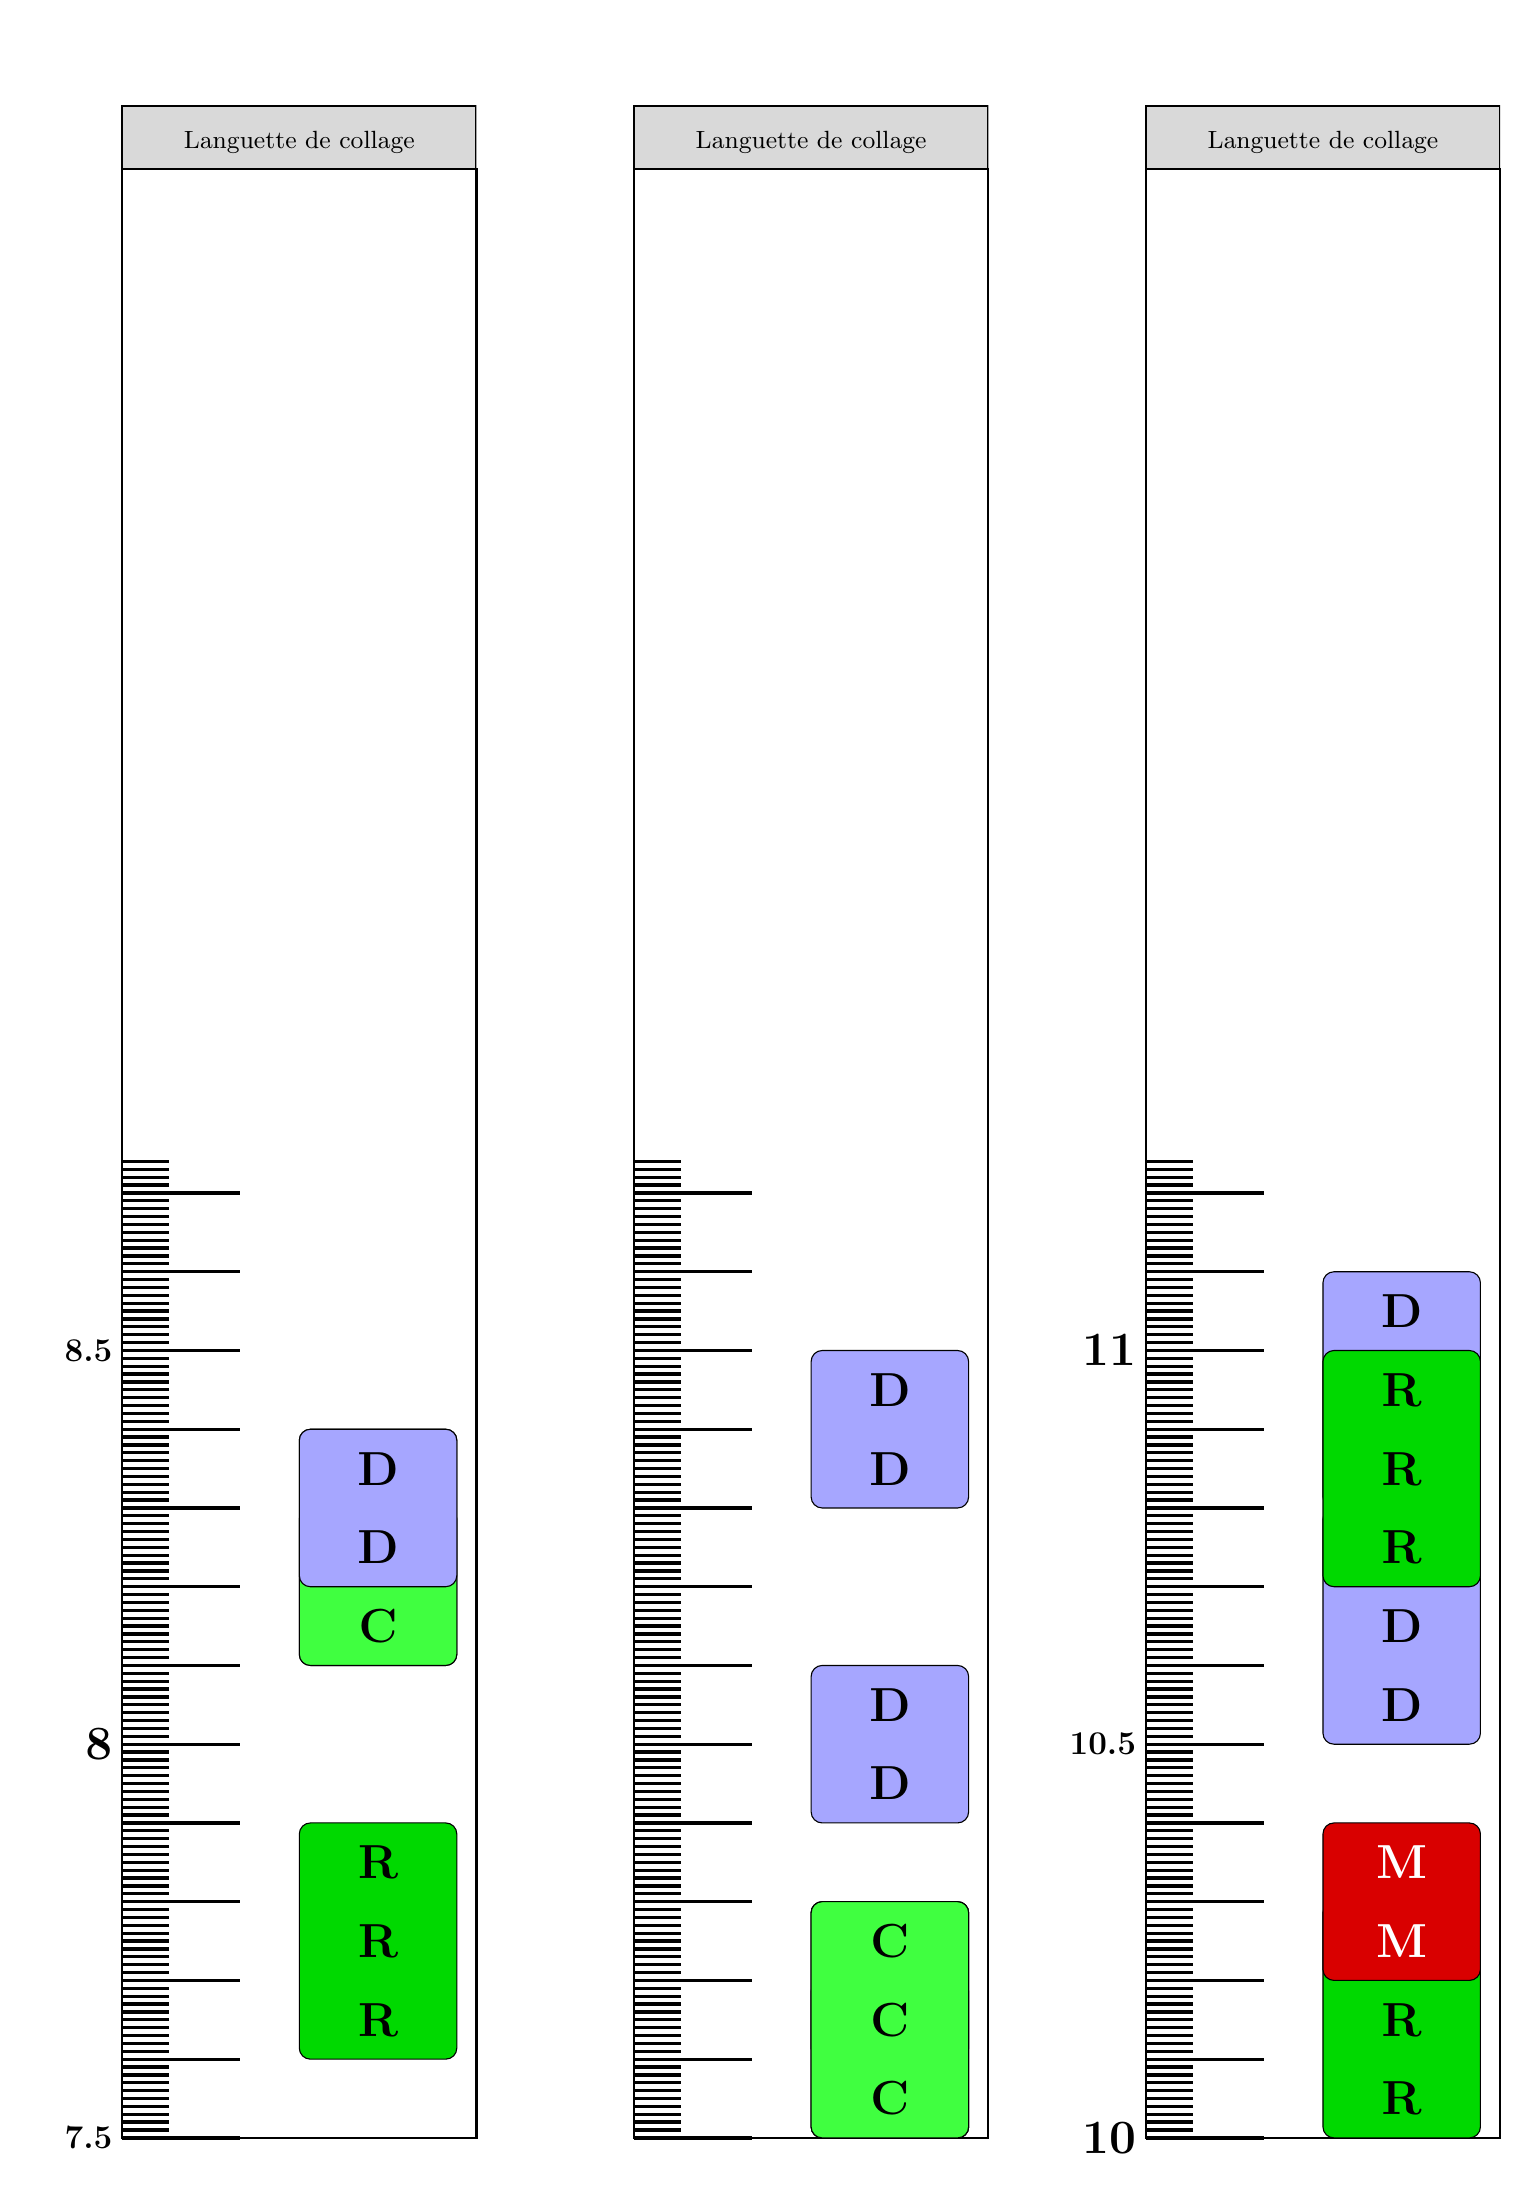
\begin{tikzpicture}[x=1cm, y=1cm,xshift=-1cm]

% Dessin de la première bande
\begin{scope}[shift={(-1,0)}]
    \draw[thick] (0,0) rectangle (\bandwidth, \bandheight);
    \clip (-1.2,-0.5) rectangle (\bandwidth, \bandheight+\languette+1);
    \drawGraduations{0}{12.5}{75}{0}
\end{scope}

% Dessin de la deuxième bande (avec continuité des nombres)
\begin{scope}[shift={(1*\bandwidth + 1,0)}]
    \draw[thick] (0,0) rectangle (\bandwidth, \bandheight);
    \clip (-1.2,-0.5) rectangle (\bandwidth, \bandheight+\languette+1);
    \drawGraduations{0}{12.5}{87.5}{0.5}
\end{scope}

% Dessin de la troisième bande (avec continuité des nombres)
\begin{scope}[shift={(2*\bandwidth + 3,0)}]
    \draw[thick] (0,0) rectangle (\bandwidth, \bandheight);
    \clip (-1.2,-0.5) rectangle (\bandwidth, \bandheight+\languette+1);
    \drawGraduations{0}{12.5}{100}{0}
\end{scope}

\end{tikzpicture}

\newpage

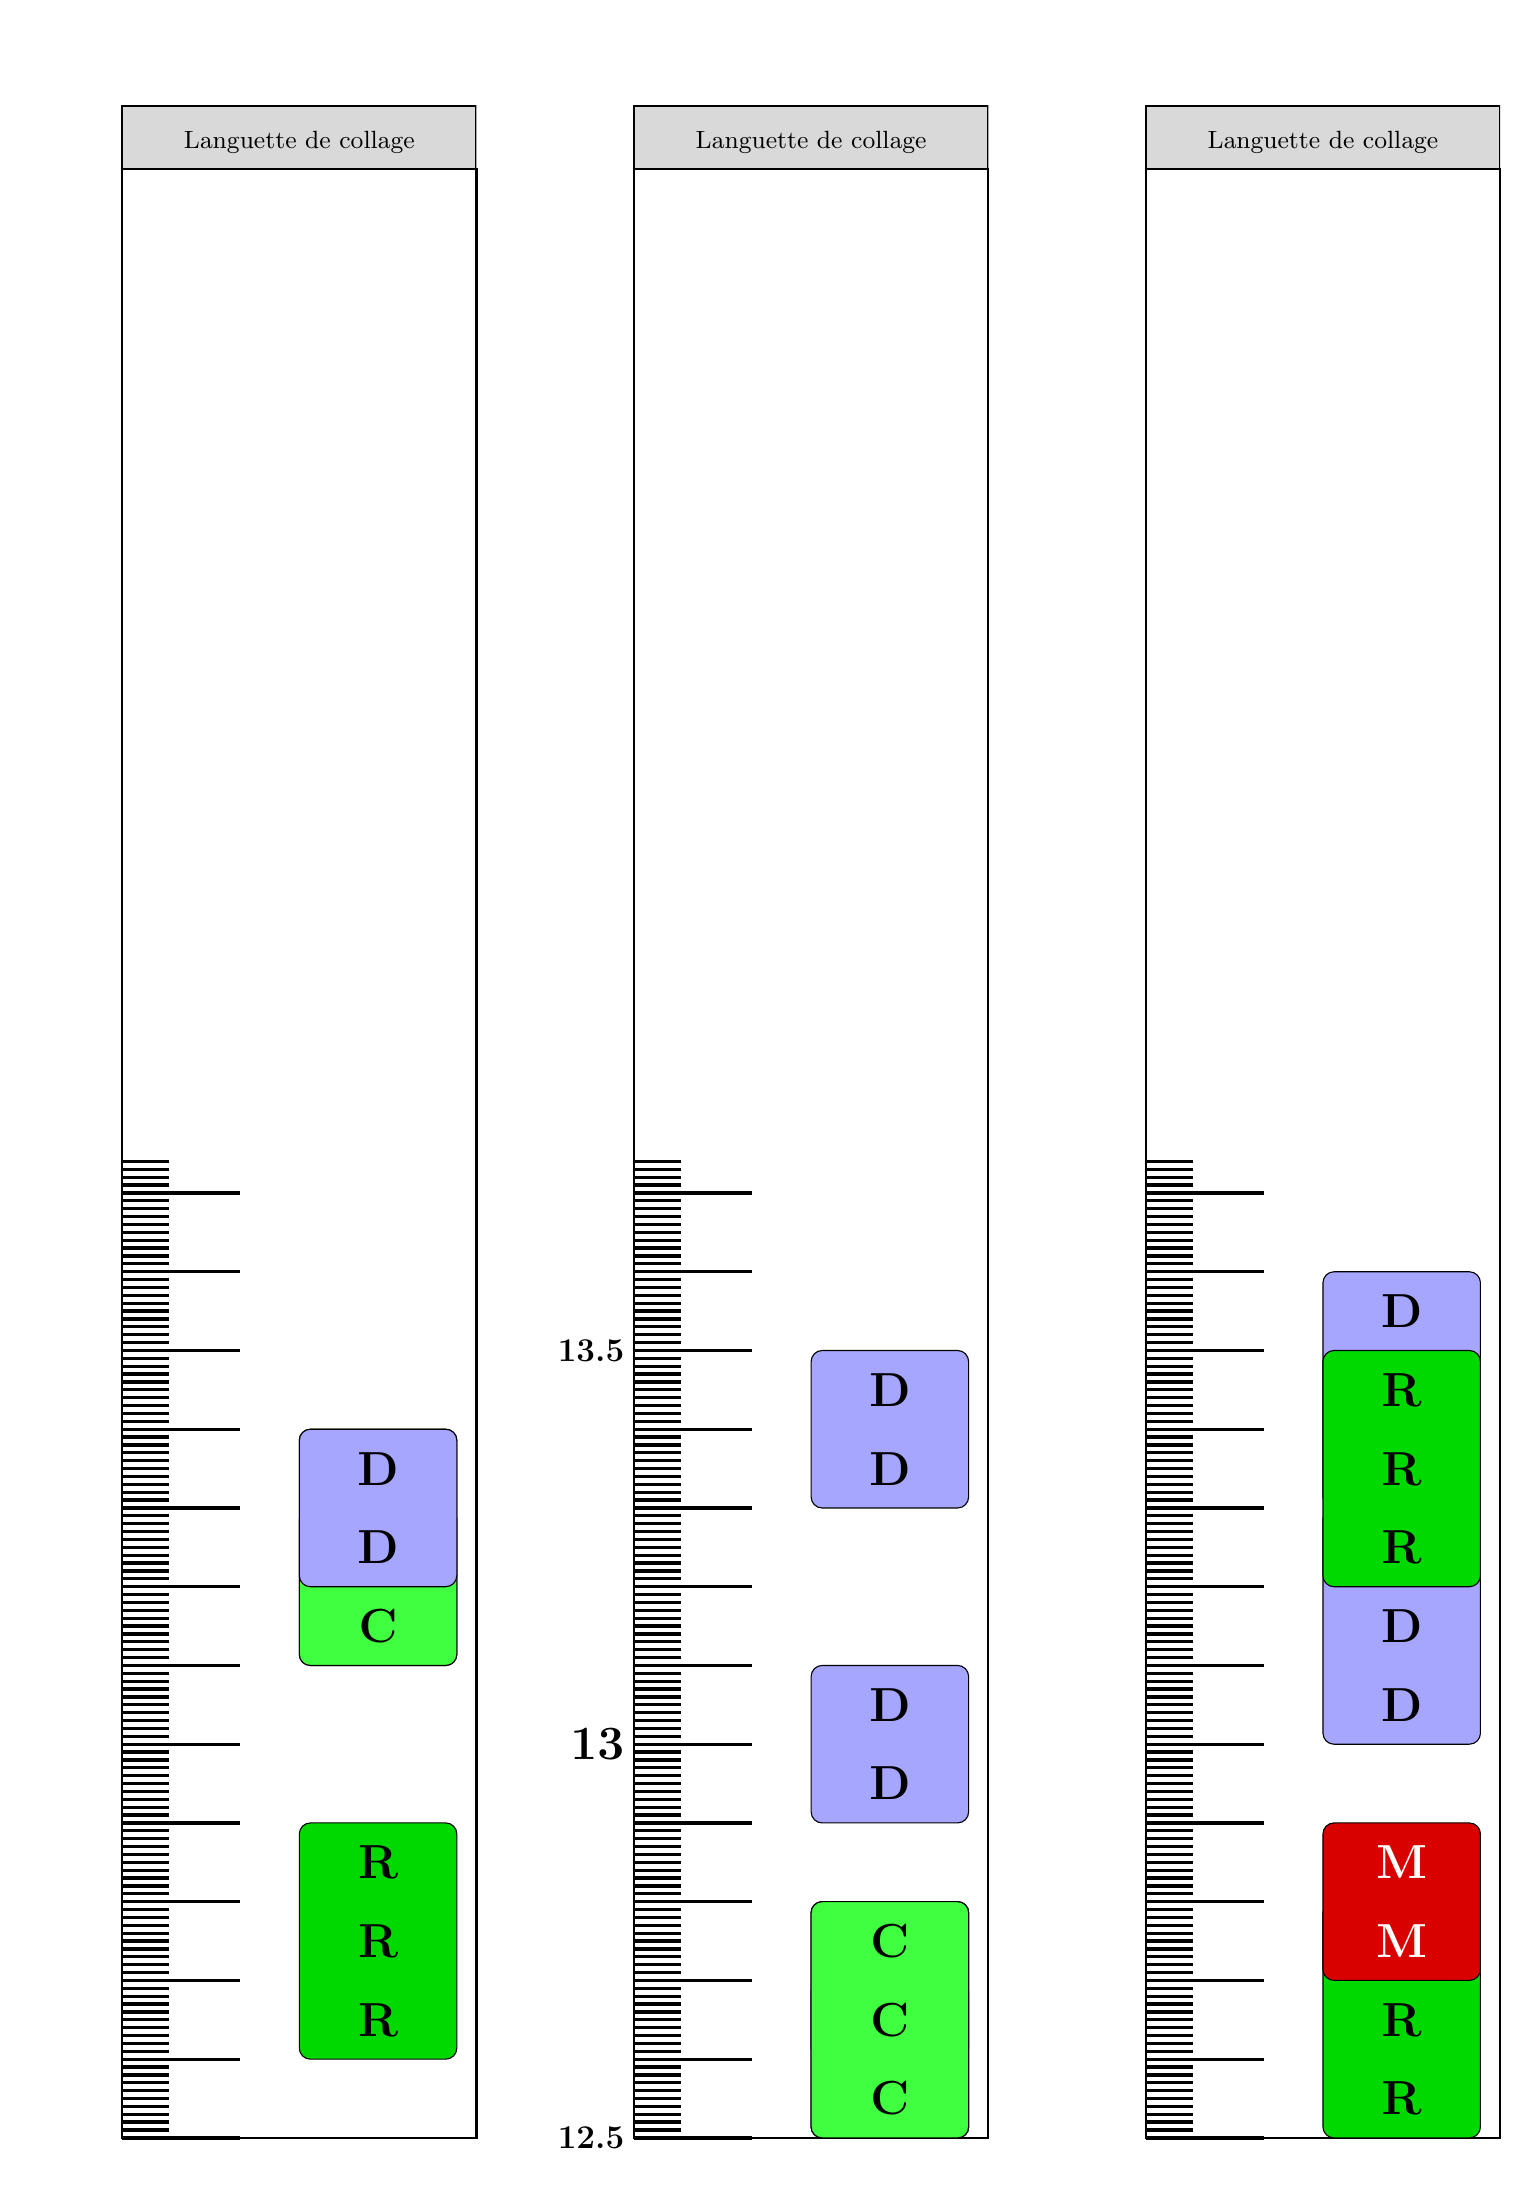
\begin{tikzpicture}[x=1cm, y=1cm,xshift=-1cm]
% Dessin de la première bande
\begin{scope}[shift={(-1,0)}]
    \draw[thick] (0,0) rectangle (\bandwidth, \bandheight);
    \clip (-1.2,-0.5) rectangle (\bandwidth, \bandheight+\languette+1);
    \drawGraduations{0}{12.5}{112.5}{0.5}
\end{scope}

% Dessin de la deuxième bande (avec continuité des nombres)
\begin{scope}[shift={(1*\bandwidth + 1,0)}]
    \draw[thick] (0,0) rectangle (\bandwidth, \bandheight);
    \clip (-1.2,-0.5) rectangle (\bandwidth, \bandheight+\languette+1);
    \drawGraduations{0}{12.5}{125}{0}
\end{scope}

% Dessin de la troisième bande (avec continuité des nombres)
\begin{scope}[shift={(2*\bandwidth + 3,0)}]
    \draw[thick] (0,0) rectangle (\bandwidth, \bandheight);
    \clip (-1.2,-0.5) rectangle (\bandwidth, \bandheight+\languette+1);
    \drawGraduations{0}{12.5}{137.5}{0.5}
\end{scope}

\end{tikzpicture}